% UrbanFix -- IEEE Access manuscript, first revision (LaTeX)
% Compile with the official IEEE Access LaTeX template files (ieeeaccess.cls,
% spotcolor.sty, logos and fonts from ieeeaccess.ieee.org) in the same folder,
% with pdfLaTeX (Overleaf: "IEEE Access LaTeX Template" project).
%
% Every number in this file comes from generated/numbers.tex or a
% generated/tab_*.tex table, written by ../scripts/build_paper_data.py from the
% committed result files. Do not type numbers from results into this file.
% ieeeaccess.cls redefines the TeX primitive \year, which TikZ needs while it loads.
% Keep the primitive, give it back to TikZ, then restore the class's \year.
\let\primitiveyear\year
\documentclass{ieeeaccess}
\usepackage{cite}
\usepackage{amsmath,amssymb,amsfonts}
\usepackage{graphicx}
\usepackage{textcomp}
\usepackage{booktabs}
\usepackage{array}
\usepackage{url}
\let\classyear\year
\let\year\primitiveyear
\usepackage{tikz}
\usetikzlibrary{arrows.meta,shapes.geometric,calc}
\let\year\classyear
% pgf replaces the page resources that hold the class's PANTONE 3015 C spot colour,
% so viewers report "Bad color space". Use the same CMYK values as a process colour.
\definecolor{accessblue}{cmyk}{1,0.3,0,0.2}

% Generated by scripts/build_paper_data.py from the committed result files. Do not edit.
\newcommand{\nPotholeSplit}{2,836/606/604}
\newcommand{\nLitterSplit}{1,000/214/214}
\newcommand{\nGraffitiSplit}{670/143/209}
\newcommand{\nPotholeNoIndiaSplit}{1,498/319/318}
\newcommand{\nExtRoboflow}{297}
\newcommand{\nExtIndiaAll}{1,911}
\newcommand{\nExtIndiaTest}{286}
\newcommand{\nExtTacoUnofficial}{2,308}
\newcommand{\nSplitSharedGroups}{0}
\newcommand{\nStormBlack}{138}
\newcommand{\nStormTotal}{1,022}
\newcommand{\nStormBlackTest}{24}
\newcommand{\nStormTest}{209}
\newcommand{\nOldManholeVal}{480}
\newcommand{\nOldManholeLeak}{262}
\newcommand{\nOldManholeCopies}{368}
\newcommand{\nHammingSixtyfour}{10}
\newcommand{\nHammingTwofivesix}{24}
\newcommand{\nPotholeTestMap}{0.516}
\newcommand{\nPotholeTestMapLo}{0.484}
\newcommand{\nPotholeTestMapHi}{0.556}
\newcommand{\nPotholeValMap}{0.526}
\newcommand{\nPotholeRecall}{0.493}
\newcommand{\nPotholePrecision}{0.593}
\newcommand{\nPotholeBestEpoch}{39}
\newcommand{\nPotholeCpuMs}{24.3}
\newcommand{\nPotholeMb}{6.2}
\newcommand{\nLitterTestMap}{0.456}
\newcommand{\nLitterTestMapLo}{0.393}
\newcommand{\nLitterTestMapHi}{0.524}
\newcommand{\nLitterValMap}{0.451}
\newcommand{\nLitterRecall}{0.403}
\newcommand{\nLitterPrecision}{0.651}
\newcommand{\nLitterBestEpoch}{39}
\newcommand{\nLitterCpuMs}{23.7}
\newcommand{\nLitterMb}{6.8}
\newcommand{\nLitterMaskMap}{0.440}
\newcommand{\nGraffitiTestMap}{0.708}
\newcommand{\nGraffitiTestMapLo}{0.654}
\newcommand{\nGraffitiTestMapHi}{0.771}
\newcommand{\nGraffitiValMap}{0.655}
\newcommand{\nGraffitiRecall}{0.650}
\newcommand{\nGraffitiPrecision}{0.718}
\newcommand{\nGraffitiBestEpoch}{40}
\newcommand{\nGraffitiCpuMs}{19.5}
\newcommand{\nGraffitiMb}{6.2}
\newcommand{\nMaxEpochs}{40}
\newcommand{\nPatience}{10}
\newcommand{\nImgSize}{640}
\newcommand{\nBatch}{16}
\newcommand{\nBootstrap}{1000}
\newcommand{\nCpuMsMin}{19.5}
\newcommand{\nCpuMsMax}{24.3}
\newcommand{\nPotholeYolovEightnMap}{0.659}
\newcommand{\nPotholeYolovEightnMapLo}{0.608}
\newcommand{\nPotholeYolovEightnMapHi}{0.710}
\newcommand{\nPotholeYolovEightnCpuMs}{24}
\newcommand{\nPotholeYolovEightnMb}{6.2}
\newcommand{\nPotholeYolovEightnWrongPass}{7.5}
\newcommand{\nPotholeYolovEightnUnrelatedPass}{1.6}
\newcommand{\nPotholeYoloOneOnenMap}{0.645}
\newcommand{\nPotholeYoloOneOnenMapLo}{0.593}
\newcommand{\nPotholeYoloOneOnenMapHi}{0.697}
\newcommand{\nPotholeYoloOneOnenCpuMs}{25}
\newcommand{\nPotholeYoloOneOnenMb}{5.5}
\newcommand{\nPotholeYoloOneOnenWrongPass}{10.3}
\newcommand{\nPotholeYoloOneOnenUnrelatedPass}{0.4}
\newcommand{\nPotholeRtdetrLMap}{0.683}
\newcommand{\nPotholeRtdetrLMapLo}{0.634}
\newcommand{\nPotholeRtdetrLMapHi}{0.733}
\newcommand{\nPotholeRtdetrLCpuMs}{349}
\newcommand{\nPotholeRtdetrLMb}{66.2}
\newcommand{\nPotholeRtdetrLWrongPass}{9.3}
\newcommand{\nPotholeRtdetrLUnrelatedPass}{1.9}
\newcommand{\nLitterYolovEightnMap}{0.456}
\newcommand{\nLitterYolovEightnMapLo}{0.393}
\newcommand{\nLitterYolovEightnMapHi}{0.524}
\newcommand{\nLitterYolovEightnCpuMs}{24}
\newcommand{\nLitterYolovEightnMb}{6.8}
\newcommand{\nLitterYolovEightnWrongPass}{15.7}
\newcommand{\nLitterYolovEightnUnrelatedPass}{28.2}
\newcommand{\nLitterYoloOneOnenMap}{0.445}
\newcommand{\nLitterYoloOneOnenMapLo}{0.382}
\newcommand{\nLitterYoloOneOnenMapHi}{0.513}
\newcommand{\nLitterYoloOneOnenCpuMs}{24}
\newcommand{\nLitterYoloOneOnenMb}{6.0}
\newcommand{\nLitterYoloOneOnenWrongPass}{15.0}
\newcommand{\nLitterYoloOneOnenUnrelatedPass}{25.9}
\newcommand{\nLitterRtdetrLMap}{0.512}
\newcommand{\nLitterRtdetrLMapLo}{0.453}
\newcommand{\nLitterRtdetrLMapHi}{0.579}
\newcommand{\nLitterRtdetrLCpuMs}{353}
\newcommand{\nLitterRtdetrLMb}{66.2}
\newcommand{\nLitterRtdetrLWrongPass}{27.0}
\newcommand{\nLitterRtdetrLUnrelatedPass}{47.7}
\newcommand{\nLitterYolovEightnSuperMap}{0.425}
\newcommand{\nLitterYolovEightnSuperMapLo}{0.365}
\newcommand{\nLitterYolovEightnSuperMapHi}{0.489}
\newcommand{\nLitterYolovEightnSuperCpuMs}{24}
\newcommand{\nLitterYolovEightnSuperMb}{6.8}
\newcommand{\nLitterYolovEightnSuperWrongPass}{32.1}
\newcommand{\nLitterYolovEightnSuperUnrelatedPass}{52.7}
\newcommand{\nGraffitiYolovEightnMap}{0.708}
\newcommand{\nGraffitiYolovEightnMapLo}{0.654}
\newcommand{\nGraffitiYolovEightnMapHi}{0.771}
\newcommand{\nGraffitiYolovEightnCpuMs}{20}
\newcommand{\nGraffitiYolovEightnMb}{6.2}
\newcommand{\nGraffitiYolovEightnWrongPass}{0.4}
\newcommand{\nGraffitiYolovEightnUnrelatedPass}{1.6}
\newcommand{\nGraffitiYoloOneOnenMap}{0.692}
\newcommand{\nGraffitiYoloOneOnenMapLo}{0.633}
\newcommand{\nGraffitiYoloOneOnenMapHi}{0.765}
\newcommand{\nGraffitiYoloOneOnenCpuMs}{20}
\newcommand{\nGraffitiYoloOneOnenMb}{5.5}
\newcommand{\nGraffitiYoloOneOnenWrongPass}{4.5}
\newcommand{\nGraffitiYoloOneOnenUnrelatedPass}{6.2}
\newcommand{\nGraffitiRtdetrLMap}{0.801}
\newcommand{\nGraffitiRtdetrLMapLo}{0.754}
\newcommand{\nGraffitiRtdetrLMapHi}{0.853}
\newcommand{\nGraffitiRtdetrLCpuMs}{349}
\newcommand{\nGraffitiRtdetrLMb}{66.2}
\newcommand{\nGraffitiRtdetrLWrongPass}{1.8}
\newcommand{\nGraffitiRtdetrLUnrelatedPass}{5.0}
\newcommand{\nGraffitiYolovEightnScratchMap}{0.457}
\newcommand{\nGraffitiYolovEightnScratchMapLo}{0.394}
\newcommand{\nGraffitiYolovEightnScratchMapHi}{0.532}
\newcommand{\nGraffitiYolovEightnScratchCpuMs}{20}
\newcommand{\nGraffitiYolovEightnScratchMb}{6.2}
\newcommand{\nGraffitiYolovEightnScratchWrongPass}{17.2}
\newcommand{\nGraffitiYolovEightnScratchUnrelatedPass}{22.9}
\newcommand{\nLitterSuperMaskMap}{0.409}
\newcommand{\nPotholeTau}{0.40}
\newcommand{\nPotholeFlag}{27.1}
\newcommand{\nPotholeFlagN}{247}
\newcommand{\nPotholeFlagTwentyfive}{11.7}
\newcommand{\nPotholeWrong}{9.3}
\newcommand{\nPotholeWrongN}{214}
\newcommand{\nPotholeWrongTwentyfive}{15.9}
\newcommand{\nPotholeUnrelated}{3.1}
\newcommand{\nPotholeUnrelatedN}{258}
\newcommand{\nPotholeUnrelatedTwentyfive}{5.4}
\newcommand{\nPotholeRoadPass}{6.2}
\newcommand{\nPotholeRoadPassN}{64}
\newcommand{\nPotholeSimFlagged}{33.8}
\newcommand{\nPotholeSimValidFlagged}{24.4}
\newcommand{\nPotholeSimInvalidPassed}{0.6}
\newcommand{\nPotholeImageRecall}{52.5}
\newcommand{\nLitterTau}{0.80}
\newcommand{\nLitterFlag}{11.5}
\newcommand{\nLitterFlagN}{104}
\newcommand{\nLitterFlagTwentyfive}{1.0}
\newcommand{\nLitterWrong}{15.7}
\newcommand{\nLitterWrongN}{287}
\newcommand{\nLitterWrongTwentyfive}{81.5}
\newcommand{\nLitterUnrelated}{28.2}
\newcommand{\nLitterUnrelatedN}{220}
\newcommand{\nLitterUnrelatedTwentyfive}{94.1}
\newcommand{\nLitterSimFlagged}{18.2}
\newcommand{\nLitterSimValidFlagged}{10.4}
\newcommand{\nLitterSimInvalidPassed}{2.2}
\newcommand{\nLitterImageRecall}{65.9}
\newcommand{\nGraffitiTau}{0.85}
\newcommand{\nGraffitiFlag}{20.0}
\newcommand{\nGraffitiFlagN}{100}
\newcommand{\nGraffitiFlagTwentyfive}{2.0}
\newcommand{\nGraffitiWrong}{0.4}
\newcommand{\nGraffitiWrongN}{289}
\newcommand{\nGraffitiWrongTwentyfive}{47.4}
\newcommand{\nGraffitiUnrelated}{1.6}
\newcommand{\nGraffitiUnrelatedN}{258}
\newcommand{\nGraffitiUnrelatedTwentyfive}{52.7}
\newcommand{\nGraffitiSimFlagged}{27.9}
\newcommand{\nGraffitiSimValidFlagged}{18.0}
\newcommand{\nGraffitiSimInvalidPassed}{0.1}
\newcommand{\nGraffitiImageRecall}{60.3}
\newcommand{\nFlagMin}{11.5}
\newcommand{\nFlagMax}{27.1}
\newcommand{\nMaxFalseFlagRule}{20}
\newcommand{\nGeoJapanMapNo}{0.629}
\newcommand{\nGeoJapanMapWith}{0.612}
\newcommand{\nGeoJapanFlagNo}{17.7}
\newcommand{\nGeoJapanFlagWith}{17.7}
\newcommand{\nGeoJapanFlagN}{96}
\newcommand{\nGeoCzechMapNo}{0.343}
\newcommand{\nGeoCzechMapWith}{0.318}
\newcommand{\nGeoCzechFlagNo}{54.5}
\newcommand{\nGeoCzechFlagWith}{81.8}
\newcommand{\nGeoCzechFlagN}{11}
\newcommand{\nGeoChinaMapNo}{0.956}
\newcommand{\nGeoChinaMapWith}{0.952}
\newcommand{\nGeoChinaFlagNo}{0.0}
\newcommand{\nGeoChinaFlagWith}{7.7}
\newcommand{\nGeoChinaFlagN}{13}
\newcommand{\nGeoIndiaMapNo}{0.113}
\newcommand{\nGeoIndiaMapWith}{0.404}
\newcommand{\nGeoIndiaFlagNo}{65.2}
\newcommand{\nGeoIndiaFlagWith}{34.8}
\newcommand{\nGeoIndiaFlagN}{115}
\newcommand{\nGeoIndiaImages}{286}
\newcommand{\nGeoIndiaFlagNoLo}{56.1}
\newcommand{\nGeoIndiaFlagNoHi}{73.3}
\newcommand{\nGeoIndiaFlagWithLo}{26.7}
\newcommand{\nGeoIndiaFlagWithHi}{43.9}
\newcommand{\nGeoIndiaRtdetrL}{0.124}
\newcommand{\nGeoIndiaYoloOneOnen}{0.096}
\newcommand{\nGeoIndiaAllMap}{0.125}
\newcommand{\nRoboflowMapNo}{0.171}
\newcommand{\nRoboflowMapWith}{0.269}
\newcommand{\nRoboflowFlag}{33.3}
\newcommand{\nTacoUnofficialMap}{0.410}
\newcommand{\nTacoUnofficialFlag}{22.5}
\newcommand{\nChiRows}{143,447}
\newcommand{\nChiWards}{50}
\newcommand{\nChiWardMedian}{2,371}
\newcommand{\nChiDuplicates}{18,955}
\newcommand{\nChiPothole}{36,489}
\newcommand{\nChiGraffiti}{95,331}
\newcommand{\nChiGarbageLitter}{11,627}
\newcommand{\nChiDraws}{200}
\newcommand{\nChiSmall}{1,000}
\newcommand{\nChiMedium}{10,000}
\newcommand{\nChiSampleWards}{10}
\newcommand{\nChiK}{5}
\newcommand{\nChiCityWithoutUrgencyAWithheld}{85.3}
\newcommand{\nChiCityWithUrgencyAWithheld}{94.2}
\newcommand{\nChiSmallWithoutUrgencyAWithheld}{100.0}
\newcommand{\nChiSmallWithUrgencyAWithheld}{100.0}
\newcommand{\nChiMediumWithoutUrgencyAWithheld}{95.1}
\newcommand{\nChiMediumWithUrgencyAWithheld}{99.4}
\newcommand{\nChiCityKOneA}{77.4}
\newcommand{\nChiSmallSingledA}{71.0}
\newcommand{\nChiSmallLearnsAfterA}{0.0}
\newcommand{\nChiSmallKOneA}{95.6}
\newcommand{\nChiCityWithoutUrgencyBWithheld}{49.1}
\newcommand{\nChiCityWithUrgencyBWithheld}{77.4}
\newcommand{\nChiSmallWithoutUrgencyBWithheld}{99.5}
\newcommand{\nChiSmallWithUrgencyBWithheld}{100.0}
\newcommand{\nChiMediumWithoutUrgencyBWithheld}{77.2}
\newcommand{\nChiMediumWithUrgencyBWithheld}{95.2}
\newcommand{\nChiCityKOneB}{21.3}
\newcommand{\nChiSmallSingledB}{71.0}
\newcommand{\nChiSmallLearnsAfterB}{0.0}
\newcommand{\nChiSmallKOneB}{81.8}
\newcommand{\nChiCityWithoutUrgencyCWithheld}{30.9}
\newcommand{\nChiCityWithUrgencyCWithheld}{51.3}
\newcommand{\nChiSmallWithoutUrgencyCWithheld}{96.5}
\newcommand{\nChiSmallWithUrgencyCWithheld}{100.0}
\newcommand{\nChiMediumWithoutUrgencyCWithheld}{50.8}
\newcommand{\nChiMediumWithUrgencyCWithheld}{77.5}
\newcommand{\nChiCityKOneC}{14.1}
\newcommand{\nChiSmallSingledC}{31.3}
\newcommand{\nChiSmallLearnsAfterC}{0.0}
\newcommand{\nChiSmallKOneC}{63.4}
\newcommand{\nChiCityWithoutUrgencyDWithheld}{12.8}
\newcommand{\nChiCityWithUrgencyDWithheld}{31.4}
\newcommand{\nChiSmallWithoutUrgencyDWithheld}{88.4}
\newcommand{\nChiSmallWithUrgencyDWithheld}{99.0}
\newcommand{\nChiMediumWithoutUrgencyDWithheld}{30.5}
\newcommand{\nChiMediumWithUrgencyDWithheld}{57.3}
\newcommand{\nChiCityKOneD}{2.9}
\newcommand{\nChiSmallSingledD}{31.3}
\newcommand{\nChiSmallLearnsAfterD}{1.0}
\newcommand{\nChiSmallKOneD}{44.8}
\newcommand{\nChiCityWithoutUrgencyEWithheld}{2.7}
\newcommand{\nChiCityWithUrgencyEWithheld}{10.0}
\newcommand{\nChiSmallWithoutUrgencyEWithheld}{52.1}
\newcommand{\nChiSmallWithUrgencyEWithheld}{82.1}
\newcommand{\nChiMediumWithoutUrgencyEWithheld}{9.6}
\newcommand{\nChiMediumWithUrgencyEWithheld}{25.7}
\newcommand{\nChiCityKOneE}{0.6}
\newcommand{\nChiSmallSingledE}{7.7}
\newcommand{\nChiSmallLearnsAfterE}{17.6}
\newcommand{\nChiSmallKOneE}{19.7}
\newcommand{\nChiCityWithoutUrgencyFWithheld}{0.3}
\newcommand{\nChiCityWithUrgencyFWithheld}{2.3}
\newcommand{\nChiSmallWithoutUrgencyFWithheld}{34.8}
\newcommand{\nChiSmallWithUrgencyFWithheld}{73.7}
\newcommand{\nChiMediumWithoutUrgencyFWithheld}{2.0}
\newcommand{\nChiMediumWithUrgencyFWithheld}{10.3}
\newcommand{\nChiCityKOneF}{0.1}
\newcommand{\nChiSmallSingledF}{7.7}
\newcommand{\nChiSmallLearnsAfterF}{26.3}
\newcommand{\nChiSmallKOneF}{8.2}
\newcommand{\nChiCityWithoutUrgencyGWithheld}{0.7}
\newcommand{\nChiCityWithUrgencyGWithheld}{2.9}
\newcommand{\nChiSmallWithoutUrgencyGWithheld}{29.1}
\newcommand{\nChiSmallWithUrgencyGWithheld}{54.0}
\newcommand{\nChiMediumWithoutUrgencyGWithheld}{2.7}
\newcommand{\nChiMediumWithUrgencyGWithheld}{10.5}
\newcommand{\nChiCityKOneG}{0.1}
\newcommand{\nChiSmallSingledG}{1.6}
\newcommand{\nChiSmallLearnsAfterG}{42.1}
\newcommand{\nChiSmallKOneG}{8.2}
\newcommand{\nChiCityWithoutUrgencyHWithheld}{0.1}
\newcommand{\nChiCityWithUrgencyHWithheld}{0.4}
\newcommand{\nChiSmallWithoutUrgencyHWithheld}{11.8}
\newcommand{\nChiSmallWithUrgencyHWithheld}{35.8}
\newcommand{\nChiMediumWithoutUrgencyHWithheld}{0.3}
\newcommand{\nChiMediumWithUrgencyHWithheld}{2.0}
\newcommand{\nChiCityKOneH}{0.0}
\newcommand{\nChiSmallSingledH}{1.6}
\newcommand{\nChiSmallLearnsAfterH}{64.0}
\newcommand{\nChiSmallKOneH}{1.9}
\newcommand{\nChiHWithheldLo}{30.9}
\newcommand{\nChiHWithheldHi}{42.0}
\newcommand{\nChiAfterMax}{0.0}
\newcommand{\nChiCellsCity}{3.0}
\newcommand{\nChiCellsSmall}{70.2}
\newcommand{\nChiCellsMedium}{17.9}
\newcommand{\nChiChosen}{H}
\newcommand{\nTestsBackend}{69}
\newcommand{\nTestsBackendPassed}{68}
\newcommand{\nTestsBackendSkipped}{1}
\newcommand{\nTestsService}{10}
\newcommand{\nTestsServicePassed}{10}
\newcommand{\nLoadFile}{2026-11-27T17-38-29-761Z.json}
\newcommand{\nLoadComplaints}{10,000}
\newcommand{\nLoadDuration}{60}
\newcommand{\nLoadCpu}{Apple M5}
\newcommand{\nLoadImageKb}{263}
\newcommand{\nLoadRegistryListFiveZerorps}{1,575}
\newcommand{\nLoadRegistryListFiveZeropfifty}{32}
\newcommand{\nLoadRegistryListFiveZeropninetynine}{45}
\newcommand{\nLoadRegistryListFiveZeroerrors}{0.0}
\newcommand{\nLoadTrackerLookupFiveZerorps}{6,552}
\newcommand{\nLoadTrackerLookupFiveZeropfifty}{7}
\newcommand{\nLoadTrackerLookupFiveZeropninetynine}{11}
\newcommand{\nLoadTrackerLookupFiveZeroerrors}{0.0}
\newcommand{\nLoadResearchRecordsFiveZerorps}{337}
\newcommand{\nLoadResearchRecordsFiveZeropfifty}{146}
\newcommand{\nLoadResearchRecordsFiveZeropninetynine}{179}
\newcommand{\nLoadResearchRecordsFiveZeroerrors}{0.0}
\newcommand{\nLoadRegistryListTwoZeroZerorps}{1,441}
\newcommand{\nLoadRegistryListTwoZeroZeropfifty}{139}
\newcommand{\nLoadRegistryListTwoZeroZeropninetynine}{53,340}
\newcommand{\nLoadRegistryListTwoZeroZeroerrors}{27.3}
\newcommand{\nLoadTrackerLookupTwoZeroZerorps}{5,620}
\newcommand{\nLoadTrackerLookupTwoZeroZeropfifty}{36}
\newcommand{\nLoadTrackerLookupTwoZeroZeropninetynine}{12,674}
\newcommand{\nLoadTrackerLookupTwoZeroZeroerrors}{2.2}
\newcommand{\nLoadResearchRecordsTwoZeroZerorps}{301}
\newcommand{\nLoadResearchRecordsTwoZeroZeropfifty}{686}
\newcommand{\nLoadResearchRecordsTwoZeroZeropninetynine}{6,024}
\newcommand{\nLoadResearchRecordsTwoZeroZeroerrors}{2.5}
\newcommand{\nLoadSubmitTwoZerorps}{40}
\newcommand{\nLoadSubmitTwoZeropfifty}{437}
\newcommand{\nLoadSubmitTwoZeropninetynine}{829}
\newcommand{\nLoadSubmitTwoZeroerrors}{0.0}
\newcommand{\nLoadSubmitBeforeRps}{4}
\newcommand{\nLoadSubmitBeforePfifty}{4,274}
\newcommand{\nLoadSubmitBeforeFile}{2026-11-24T17-44-29-345Z.json}
\newcommand{\nCostMsPerComplaint}{73}
\newcommand{\nCostPerCoreDay}{1,200,000}
\newcommand{\nCostCpgramsPerDay}{7,178}
\newcommand{\nCostCoreShare}{0.6}

% \input cannot be used inside a tabular before \bottomrule; the primitive can.
\makeatletter
\newcommand{\tablebody}[1]{\@@input #1 }
\makeatother

% filled / half / empty markers used in Table II and Table IV
\definecolor{markink}{HTML}{1F3A5F}
\definecolor{markline}{HTML}{8A94A6}
\newcommand{\yes}{\tikz[baseline=-0.6ex]\fill[markink] (0,0) circle (2.1pt);}
\newcommand{\part}{\tikz[baseline=-0.6ex]{\draw[markink,line width=0.5pt] (0,0) circle (2.1pt);\fill[markink] (0,-2.1pt) arc (-90:90:2.1pt) -- cycle;}}
\newcommand{\no}{\tikz[baseline=-0.6ex]\draw[markline,line width=0.5pt] (0,0) circle (2.1pt);}
\newcommand{\repoURL}{\url{https://github.com/pizzaparth/urbanfix}}
\newcommand{\archiveDOI}{[Zenodo DOI to be added on acceptance]}

\begin{document}
\history{Date of publication xxxx 00, 0000, date of current version xxxx 00, 0000.}
\doi{10.1109/ACCESS.2026.Doi Number}

\title{UrbanFix: A Closed-Loop Civic Complaint Platform with AI-Assisted Photo Triage, an Auditable Public Registry and Pseudonymised Research Access}

\author{\uppercase{Parth Pancholi}\authorrefmark{1},
\uppercase{Gaurav Soni}\authorrefmark{1}, \IEEEmembership{Senior Member, IEEE},
\uppercase{Kamlesh Chandravanshi}\authorrefmark{1},
\uppercase{Mahendra Sahare}\authorrefmark{2}, and
\uppercase{Jay Prakash Maurya}\authorrefmark{1}}

\address[1]{School of Computing Science and Engineering, VIT Bhopal University, Bhopal, India (e-mail: parth.25bce10443@vitbhopal.ac.in; gaurav.soni@vitbhopal.ac.in; kamlesh.chandravanshi@vitbhopal.ac.in; jpeemaurya@gmail.com)}
\address[2]{School of Computer Science and Engineering, VIT-AP University, Amaravati, India (e-mail: mahendra.sahare@vitap.ac.in)}

\markboth
{P. Pancholi \headeretal: UrbanFix: A Closed-Loop Civic Complaint Platform with AI-Assisted Photo Triage}
{P. Pancholi \headeretal: UrbanFix: A Closed-Loop Civic Complaint Platform with AI-Assisted Photo Triage}

\corresp{Corresponding author: Mahendra Sahare (e-mail: mahendra.sahare@vitap.ac.in).}

\begin{abstract}
Most digital grievance systems classify complaint text and track tickets. They rarely check the photo a citizen attaches, their urgency estimates cannot be traced to inputs, and only the administration sees the records. We present UrbanFix, an open-source civic complaint platform that follows a complaint from the citizen's photo to a publicly recorded repair and on to research data. Citizens file without an account using an email code. For potholes, litter and graffiti, a YOLOv8n detector screens the photos; when its highest confidence falls below a per-category threshold chosen on validation data, the complaint is flagged for a supervisor, never rejected. On held-out test sets, box mAP50 is \nPotholeTestMap{} (95\,\% CI \nPotholeTestMapLo--\nPotholeTestMapHi), \nLitterTestMap{} and \nGraffitiTestMap{}. On synthetic complaints built from test photos, the models flag \nPotholeFlag\,\%, \nLitterFlag\,\% and \nGraffitiFlag\,\% of valid complaints and pass \nPotholeUnrelated\,\%, \nLitterUnrelated\,\% and \nGraffitiUnrelated\,\% of unrelated ones. Adding Indian road photos to training lowered the share of valid Indian pothole complaints flagged from \nGeoIndiaFlagNo\,\% to \nGeoIndiaFlagWith\,\%. A weighted questionnaire, scored on the server, gives a traceable urgency, and a seven-state workflow enforced on the server requires ward-level assignment and photo proof before closure, then issues a receipt. Complaints are published without the filer's identity. Approved researchers receive logged, time-limited, pseudonymised records generalised to the quarter, with classes smaller than five withheld, a setting chosen by measuring linkage risk on \nChiRows{} Chicago 311 requests. The workflow results come from seeded data; the system has not been deployed.
\end{abstract}

\begin{keywords}
e-governance, civic technology, object detection, YOLOv8, human-in-the-loop AI, open government data, pseudonymisation, $k$-anonymity, audit logs
\end{keywords}

\titlepgskip=-21pt

\maketitle

\section{Introduction}

\PARstart{I}{n} India, pothole-related road accidents rose from 3,713 in 2020 to 5,432 in 2024, an increase of 46\%, and pothole-related accidents killed 8,963 people between 2018 and 2022 \cite{b1,b2}. The national grievance portal CPGRAMS received between 18.7 and 26.2 lakh grievances a year from 2019 to 2024 \cite{b3,b4}, and in FY 2023--24 State and Union Territory governments, which handle municipal complaints, took 119 days on average to dispose of one, against 16 days for central ministries \cite{b5} (Fig.~\ref{fig:f1}).

Fig.~\ref{fig:f1}(a) shows pothole accidents dipping slightly in 2021, peaking at 5,840 in 2023 and staying above 5,000 in 2024, so the problem grew over the five years. In Fig.~\ref{fig:f1}(b) the light bars are the backlog carried over from the previous year, which fell from 10.7 lakh in 2020 to 3.1 lakh in 2024; the portal now clears most of what it receives. The dark bars are new grievances, and they reached their highest value, 26.2 lakh, in the same year. Faster disposal has not reduced the number of people who need to complain, so this paper looks at what happens to a complaint after it is filed.

\begin{figure}[!tb]
\centering
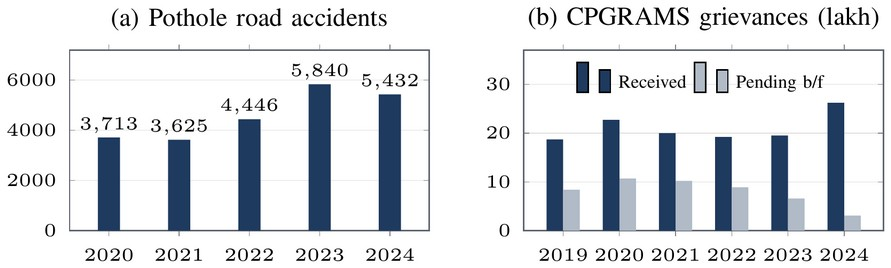
\includegraphics[width=0.89\columnwidth]{figs/fig01.jpg}
\caption{Motivation: (a) pothole-related road accidents in India \cite{b2}; (b) grievances received on CPGRAMS and the backlog brought forward each year \cite{b3,b4}.}
\label{fig:f1}
\end{figure}

Recent systems route complaint text \cite{b6,b7}, predict urgency \cite{b8}, classify waste images \cite{b9} or filter unsafe photos \cite{b10}. None of them checks whether a photo shows the reported defect or lets anyone trace an urgency label back to its inputs, and their records stay with officials or the person who filed. UrbanFix runs each complaint through a governance loop of six steps in one system (Fig.~\ref{fig:f2}).

The contribution of this paper is a system design and an open, tested implementation, together with an evaluation protocol. We do not propose a new detection model or a new privacy method. Specifically:

\begin{enumerate}
\item A complaint workflow that combines a traceable questionnaire urgency, per-category photo screening that can flag but never reject, a guarded state machine with ward-level assignment and photo proof, a public registry and a research gateway, released as open source with \nTestsBackend{} backend and \nTestsService{} vision-service tests.
\item An evaluation protocol for photo screening at the level of complaints rather than images: splits grouped by source photo, a threshold per category chosen by a written rule on validation data, test-set confidence intervals, and false-flag and false-pass rates on valid, wrong-category and unrelated complaints, with two baselines, two ablations and a cross-country test.
\item A measured privacy analysis: the linkage risk of the research release on public 311 data, which set the generalisation and the $k$-anonymity threshold now enforced by the server.
\end{enumerate}

Fig.~\ref{fig:f2} reads clockwise from the top. A citizen reports without an account, and the model for the chosen category screens the photo. A supervisor triages the complaint with the questionnaire urgency $u_Q$, the model's confidence and any review flag side by side. Field staff carry out the work inside the state machine of Eq.~(\ref{eq:fsm}) and prove the repair with photos, the citizen receives a PDF receipt, and the closed record feeds the public registry and the research data. The centre of the ring is a single complaint record. Every step reads and appends to the same document, so the history the public and researchers see is the one staff produced while working.

\begin{figure}[!tb]
\centering
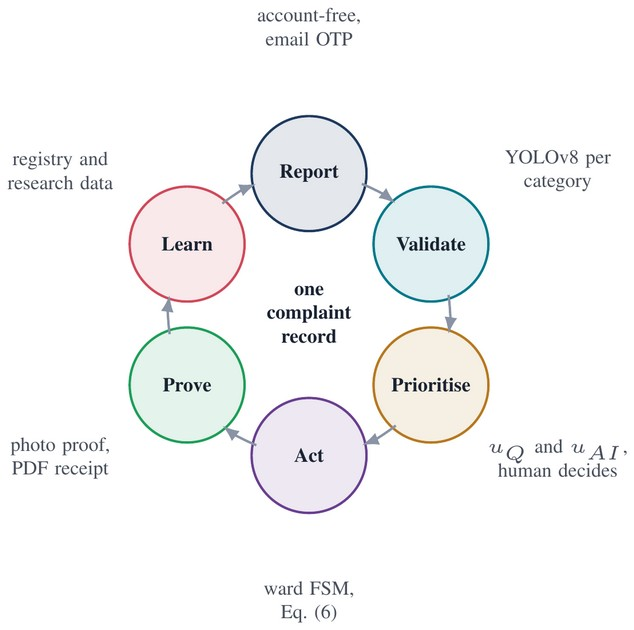
\includegraphics[width=0.63\columnwidth]{figs/fig02.jpg}
\caption{The governance loop: six steps every complaint passes through in UrbanFix.}
\label{fig:f2}
\end{figure}

\begin{table*}[!t]
\caption{Literature survey}
\label{tab:t1}
\centering
\footnotesize
\setlength{\tabcolsep}{3pt}
\renewcommand{\arraystretch}{1.1}
\begin{tabular}{@{}>{\centering\arraybackslash}p{0.035\textwidth}p{0.18\textwidth}p{0.4\textwidth}p{0.33\textwidth}@{}}
\toprule
S.No. & Authors & Work done & Limitations\\
\midrule
\multicolumn{4}{@{}l}{\textit{A. AI-assisted complaint management}}\\
1 & Chen \textit{et al.} \cite{b20}, 2022 & Treat complaint routing as text classification on real government service records, with automatic label correction that merges highly similar labels. & Complaint text only; evaluated on one partner's records.\\
2 & Javali \textit{et al.} \cite{b21}, 2025 & Infra-Alert: web portal with automatic geolocation, cloud-stored photos, before/after repair photos and PDF reports. & AI verification and prioritisation left as future work; citizens see only their own complaints.\\
3 & Vishwanath \textit{et al.} \cite{b9}, 2025 & ReGenX: Android waste app with geofenced collection alerts, an on-device complaint classifier (90.1\%) and a waste-image classifier (85.2\%). & Waste collection only; needs the app and an account; the image model sorts waste type and does not check the reported problem.\\
4 & Kanagapriya and Kesika \cite{b6}, 2026 & CitiWatch: anonymous reporting with mobile OTP; TF-IDF features and a supervised classifier route text to ten departments with 96.8\% accuracy. & Phone number stays linked to each complaint; no photo evidence; no public registry.\\
5 & Cholke \textit{et al.} \cite{b8}, 2026 & VidyutSaathi: Sentence-BERT multi-task network for severity and resolution time, DBSCAN duplicate clustering and workload-aware assignment, tested on over 20,000 electricity complaints. & Electricity complaints only; urgency is a network output the citizen cannot trace; no public view.\\
6 & Salunkhe \textit{et al.} \cite{b10}, 2026 & CivicMate: photo upload with automatic location, SMS updates and community upvoting; NudeNet screens photos for unsafe content (F1 0.97). & Screening only checks that an image is safe, so a photo of something else still passes; registration required.\\
7 & Katkar \textit{et al.} \cite{b22}, 2026 & CivicX: grievance routing with geospatial heat maps plus ML screening of building plans; 91.4\% classification accuracy against 94.1\% for officers. & Below manual accuracy; transparency limited to officials' dashboards; photos not checked against the complaint.\\
8 & Praveen Kumar \textit{et al.} \cite{b7}, 2026 & Smart City Concern: portal and X posts routed by zero-shot BART (92.8\%), with DistilBERT sentiment for priority, OCR on photos and TF-IDF duplicate linking. & Sentiment stands in for urgency, which the authors note may not reflect real severity; official dashboard only.\\
\multicolumn{4}{@{}l}{\textit{B. Citizen reporting and 311 data}}\\
9 & King and Brown \cite{b23}, 2007 & Evaluated FixMyStreet, an early UK site where residents post local problems and follow them until they are fixed; over 3,000 reports and updates in its first six months. & Council officers reported duplicate reports, difficulty confirming fixes and managing expectations.\\
10 & Goodchild \cite{b24}, 2007 & Introduced volunteered geographic information, with citizens acting as sensors, and examined contributor motives, data accuracy and privacy. & Conceptual review; the accuracy of volunteered data is left as an open question.\\
11 & Clark \textit{et al.} \cite{b12}, 2013 & Tested one year of Boston service requests for race, education and income bias using geospatial analysis and negative binomial regression. & Poorer neighbourhoods used the service less, and Hispanic residents may use it less as requests move online.\\
\bottomrule
\end{tabular}
\end{table*}

\begin{table*}[!t]
\addtocounter{table}{-1}
\caption{Literature survey (continued)}
\centering
\footnotesize
\setlength{\tabcolsep}{3pt}
\renewcommand{\arraystretch}{1.1}
\begin{tabular}{@{}>{\centering\arraybackslash}p{0.035\textwidth}p{0.18\textwidth}p{0.4\textwidth}p{0.33\textwidth}@{}}
\toprule
S.No. & Authors & Work done & Limitations\\
\midrule
12 & Minkoff \cite{b25}, 2016 & Modelled tract-level variation in New York 311 contact volume for goods, graffiti and noise complaints with spatial regression. & Volume reflects the propensity to contact as well as conditions, which makes 311 data hard to use for locating problems.\\
13 & Pak \textit{et al.} \cite{b13}, 2017 & Compared 30,041 FixMyStreet reports from Brussels with socio-demographic statistics and geotagged Twitter data. & Use varied by district, and low-income and ethnically diverse communities were under-represented among those reporting.\\
14 & Wang \textit{et al.} \cite{b26}, 2017 & Showed that the mix of 311 request types in New York, Boston and Chicago acts as a neighbourhood signature that groups areas by socio-economic profile. & Uses aggregate request counts for planning; individual complaints are not handled.\\
15 & Kontokosta and Hong \cite{b14}, 2021 & Linked Kansas City 311 reports with a resident survey, code violations and street assessments to classify neighbourhoods as under- or over-reporting. & Low-income and minority areas reported street issues less despite greater need, so decisions driven by complaint counts can be unfair.\\
\multicolumn{4}{@{}l}{\textit{C. Vision models for civic defects}}\\
16 & Redmon \textit{et al.} \cite{b27}, 2016 & YOLO: one network predicts boxes and classes for the whole image in a single pass, at 45 frames/s (155 for Fast YOLO). & More localisation errors than the strongest detectors of the time.\\
17 & Maeda \textit{et al.} \cite{b28}, 2018 & 9,053 smartphone images from seven Japanese municipalities with 15,435 instances of eight road-damage types; detector run on a GPU server and a smartphone. & Japanese roads only; road damage only.\\
18 & Dhiman and Klette \cite{b29}, 2020 & Reviewed pothole detection and compared two stereo-vision methods with two deep-learning models for the road ahead of a vehicle. & Designed for vehicle cameras; potholes only.\\
19 & Fan \textit{et al.} \cite{b30}, 2020 & Transform a dense disparity map and fit a quadratic road surface to find potholes, at about 98.7\% pixel-level accuracy. & Needs stereo disparity input; potholes only.\\
20 & Arya \textit{et al.} \cite{b31}, 2021 & 26,620 smartphone images from several countries; tested whether a model trained in Japan transfers and proposed generalised models. & Road damage only; detections are not linked to complaint handling.\\
21 & Córdova \textit{et al.} \cite{b32}, 2022 & Compared five detector families on the new PlastOPol set (2,418 images) and TACO; YOLOv5x reached AP50 of 84.9 and 63.3, and YOLOv5s ran on a phone. & All models struggled with small items such as cigarette butts and gave false positives on natural backgrounds.\\
22 & Fogaça \textit{et al.} \cite{b33}, 2023 & Lisbon images classified as illegal graffiti, street art or none (81.4\% accuracy), then illegal graffiti localised (70.3\% IoU). & Weakest on images without graffiti (F1 66\%); one city.\\
\multicolumn{4}{@{}l}{\textit{D. Open data, urban computing and AI in government}}\\
23 & Janssen \textit{et al.} \cite{b34}, 2012 & Used interviews and a workshop to list what open data offers and what holds back its use, and set out five myths about it. & Finds that publishing data is often assumed to bring use and benefit by itself; qualitative study.\\
24 & Zheng \textit{et al.} \cite{b35}, 2014 & Reviewed how city data are collected, stored, combined and analysed, with examples from seven application areas. & Survey of methods; no complaint-handling system is proposed.\\
25 & Wirtz \textit{et al.} \cite{b36}, 2019 & Reviewed the literature to map where governments apply AI (ten areas) and what makes it hard (four groups of challenges). & Conceptual overview without implementation or evaluation.\\
\multicolumn{4}{@{}l}{\textit{E. Human oversight and privacy}}\\
26 & Sweeney \cite{b37}, 2002 & Defined $k$-anonymity, where each released record is indistinguishable from at least $k-1$ others, and examined re-identification attacks. & Releases can still be attacked when the accompanying release policies are not followed.\\
27 & Amershi \textit{et al.} \cite{b38}, 2019 & Proposed 18 guidelines for human-AI interaction and tested them with 49 practitioners on 20 AI products. & General guidelines; the study also found gaps in current knowledge.\\
28 & Wu \textit{et al.} \cite{b39}, 2022 & Surveyed human-in-the-loop machine learning, grouped by where people step in: preparing data, training the model, or designing the whole system. & Survey; identifies open challenges rather than a deployable design.\\
\bottomrule
\end{tabular}
\end{table*}

\section{Related Work}\label{sec:rw}

Table~\ref{tab:t1} groups 28 studies into five strands. Recent complaint platforms (A) route text with 90 to 97\% accuracy, yet none of them checks the photo against the reported defect. Studies of FixMyStreet and 311 data (B) find that who reports, and how often, varies with income and ethnicity \cite{b12,b13,b14}, so complaint counts alone are a biased guide to need. Detectors for road damage, potholes, litter and graffiti (C) are evaluated apart from any complaint workflow. Strands D and E cover open data, AI in government and human oversight. Table~\ref{tab:t2} compares UrbanFix with the seven platforms closest to it.

Three further bodies of work shape the design but are not complaint systems. On disclosure, $k$-anonymity \cite{b37} bounds how often a released record can be singled out, but not what an adversary learns when all matching records share a value; $l$-diversity \cite{b41} addresses that gap. Sparse records with fine location and time are easy to re-identify \cite{b43,b44,b45}, and differential privacy \cite{b42,b51} gives formal guarantees for aggregate releases at a cost in accuracy. Pseudonymisation is treated as a safeguard, not as anonymisation, by both ENISA \cite{b46} and the GDPR \cite{b47}. On accountability, role-based access control \cite{b49} and tamper-evident audit logs built on hash chains \cite{b50,b52} are standard designs, and workflow nets \cite{b53} model case handling as guarded transitions. On evaluation, detection results are reported with the PASCAL VOC and COCO average precision \cite{b54,b55}, and RT-DETR \cite{b56} is a current transformer detector that runs in real time on a GPU. Localised datasets with documented provenance and open licences now exist for road damage \cite{b15}, litter \cite{b17} and graffiti \cite{b19}.

\section{System Architecture}\label{sec:arch}

One Expo client serves all six roles, and the server decides which screens a user sees (Fig.~\ref{fig:f3}). A request passes up to seven checks before it reaches a controller (public routes have no authentication step, and rate limits apply to codes, login and filing), and the server re-checks the account, any pending invitation and research expiry on every call. Intake sends photos to a separate FastAPI service only after returning the tracking ID, so a slow or failed model call cannot affect the filing. Each MongoDB complaint document embeds its status history and AI analysis. Because the paper counts several different things, Table~\ref{tab:t3} fixes one name for each count.

\begin{figure*}[!t]
\centering
\resizebox{\textwidth}{!}{% Fig. 3: layered architecture, drawn from backend/app.js, backend/routes/,
% backend/middleware/ and ai_service/. Revised: three models, per-category tau_k,
% seven request checks, rate limits, metadata removal, hash-chained access log.
\begin{tikzpicture}[
  font=\scriptsize,
  box/.style={draw=markink, rounded corners=1.5pt, align=center, inner sep=2.5pt, minimum height=8.5mm, text width=#1},
  box/.default=19mm,
  actor/.style={draw=markline, fill=markline!12, rounded corners=1.5pt, align=center, minimum height=5mm, text width=17mm},
  lbl/.style={font=\scriptsize\bfseries, text=markline, anchor=west},
  arr/.style={-{Latex[length=1.6mm]}, markink, line width=0.5pt},
  async/.style={-{Latex[length=1.6mm]}, teal!70!black, dashed, line width=0.6pt},
]
% actors
\foreach \a [count=\i from 0] in {Citizen, Public, Supervisor, Field worker, Administrator, Researcher}
  \node[actor] (a\i) at (\i*2.95, 0) {\a};
% client
\node[draw=markink, line width=0.7pt, rounded corners=2pt, minimum width=17.6cm, minimum height=9mm, anchor=north west,
      align=left, inner sep=3pt] (client) at (-1.0,-0.65)
  {\textbf{Expo / React Native client} (Android, iOS, web): one app, five role shells chosen by the server; citizens and the public share one};
\foreach \i in {0,...,5} \draw[arr] (a\i) -- (a\i |- client.north);
% pipeline
\node[lbl] at (-1.0,-1.95) {REQUEST PIPELINE: seven checks on every call (Express)};
\foreach \t [count=\i from 0] in {
  {1 Transport\\HTTPS, CORS, body limit},
  {2 Rate limits\\OTP, login, filing},
  {3 Uploads\\$\le$3 photos, metadata removed},
  {4 Authentication\\JWT + live account check},
  {5 Authorisation\\role, scope, expiry},
  {6 Validation\\Zod schemas, consent},
  {7 Error boundary\\typed 4xx / 5xx}}
  \node[box=21mm] (p\i) at (\i*2.53, -2.75) {\t};
\foreach \i [evaluate=\i as \j using int(\i+1)] in {0,...,5} \draw[arr] (p\i) -- (p\j);
\draw[arr, <->] (client.south -| p3) -- (p3.north) node[midway, right, font=\tiny] {REST / JSON};
% services
\node[lbl] at (-1.0,-3.75) {DOMAIN SERVICES (7 routers, 59 endpoints)};
\foreach \t [count=\i from 0] in {
  {Identity\\OTP, invites},
  {Intake\\tracking ID, $U$, $u_Q$ (Eq.~\ref{eq:urg})},
  {Workflow\\guarded FSM (Eq.~\ref{eq:fsm})},
  {Workforce\\attendance, leave},
  {Transparency\\registry, tracker, receipts},
  {Analytics\\KPIs, ward monitoring},
  {Research gateway\\$\pi$, $k$-suppression, quotas}}
  \node[box=21mm] (s\i) at (\i*2.53, -4.55) {\t};
\draw[arr] (p3.south) -- ++(0,-0.25) -| (s2.north);
\draw[violet!70!black, line width=0.8pt, rounded corners=1.5pt] (s6.south west) rectangle (s6.north east);
% inference tier
\node[draw=teal!70!black, dashed, rounded corners=2pt, minimum width=8.6cm, minimum height=2.2cm, anchor=north west] (inf) at (-1.0,-5.75) {};
\node[lbl, text=teal!70!black, anchor=south west] at (inf.south west) {VISION SERVICE (FastAPI, Ultralytics)};
\node[box=13mm, fill=teal!8] (router) at (0.0,-6.7) {Category\\router};
\node[box=27mm, minimum height=5mm] (m1) at (2.65,-6.1) {pothole: YOLOv8n (box)};
\node[box=27mm, minimum height=5mm] (m2) at (2.65,-6.7) {litter: YOLOv8n-seg};
\node[box=27mm, minimum height=5mm] (m3) at (2.65,-7.3) {graffiti: YOLOv8n (box)};
\node[box=25mm, fill=teal!8] (post) at (6.1,-6.7) {$s^{*}$; $\delta$ (litter only);\\flag $r$ if $s^{*}<\tau_k$;\\annotated photos\\(Eqs.~\ref{eq:sstar}--\ref{eq:flag})};
\foreach \m in {m1,m2,m3} {\draw[arr] (router.east) -- (\m.west); \draw[arr] (\m.east) -- (post.west);}
\draw[async] ([xshift=-4mm]s1.south) -- node[left, font=\tiny, align=right] {photos, after the\\tracking ID is returned} ([xshift=-4mm]s1.south |- inf.north);
\draw[async] (post.north) -- ++(0,0.62) -| node[pos=0.25, above, font=\tiny] {\texttt{aiAnalysis} for triage} ([xshift=4mm]s1.south);
% data tier
\node[draw=orange!70!black, dashed, rounded corners=2pt, minimum width=9.0cm, minimum height=2.2cm, anchor=north west] (dat) at (7.85,-5.75) {};
\node[lbl, text=orange!70!black, anchor=south west] at (dat.south west) {DATA AND INTEGRATION};
\node[box=21mm, fill=orange!8] (db) at (9.15,-6.7) {MongoDB\\8 collections\\embedded history and AI evidence};
\node[box=17mm] (fs) at (11.35,-6.7) {Object store\\photos, proof};
\node[box=17mm] (smtp) at (13.25,-6.7) {SMTP\\codes, receipts};
\node[box=19mm] (log) at (15.3,-6.7) {Access log\\hash-chained, head hash public};
\foreach \s in {s4, s5, s6} \draw[arr, orange!70!black] (\s.south) -- (\s.south |- dat.north);
\end{tikzpicture}
}
\caption{Layered architecture of UrbanFix. Solid arrows are synchronous requests. Dashed teal arrows show the call to the vision service, made after the tracking ID has been returned. The research gateway (purple) is the only path to bulk data, and every research request is written to the hash-chained access log.}
\label{fig:f3}
\end{figure*}

\begin{table}[!tb]
\caption{Capabilities of reviewed systems and UrbanFix (UF)}
\label{tab:t2}
\centering
\footnotesize
\setlength{\tabcolsep}{3.2pt}
\begin{tabular}{@{}l*{7}{c}c@{}}
\toprule
Capability & \cite{b21} & \cite{b6} & \cite{b8} & \cite{b9} & \cite{b10} & \cite{b22} & \cite{b7} & UF\\
\midrule
Account-free filing & \no & \part & \no & \no & \no & \no & \no & \yes\\
Photo evidence & \yes & \no & \part & \yes & \yes & \yes & \part & \yes\\
Photo--defect screening & \no & \no & \part & \no & \no & \no & \no & \yes\\
Urgency scoring & \no & \no & \yes & \no & \no & \yes & \yes & \yes\\
Traceable urgency & \no & \no & \no & \no & \no & \no & \no & \yes\\
Automated routing & \part & \yes & \yes & \part & \yes & \yes & \yes & \part\\
Field proof of repair & \yes & \no & \no & \no & \no & \no & \no & \yes\\
Resolution receipt & \part & \no & \no & \no & \no & \no & \no & \yes\\
Public registry & \no & \no & \no & \no & \part & \no & \no & \yes\\
Pseudonymised research data & \no & \no & \no & \no & \no & \no & \no & \yes\\
\bottomrule
\multicolumn{9}{@{}l}{\scriptsize \yes~supported \quad \part~partial \quad \no~not supported or not reported}
\end{tabular}
\end{table}

\begin{table}[!tb]
\caption{Counts used in this paper}
\label{tab:t3}
\centering
\footnotesize
\setlength{\tabcolsep}{3pt}
\begin{tabular}{@{}p{2.1cm}cp{4.9cm}@{}}
\toprule
Term & Count & What it is\\
\midrule
Governance loop & 6 steps & Report, AI screening, triage, field work, receipt, registry and research (Fig.~\ref{fig:f2})\\
Workflow states & 7 states & sub, acc, asg, wip, prf, cls, rej (Eq.~\ref{eq:fsm}, Fig.~\ref{fig:f8})\\
Main path & 5 transitions & accept, assign, start, proof, close; plus reject and rework\\
Request checks & 7 checks & The middleware chain in front of the controllers; each route uses the checks it needs (Fig.~\ref{fig:f3})\\
Roles & 6 roles & Citizen, public, supervisor, field worker, administrator, researcher; citizens and the public share one app shell\\
\bottomrule
\end{tabular}
\end{table}

Fig.~\ref{fig:f3} reads from top to bottom. The six actors use the same client, which gives each of them one of five role shells. The request checks run in a fixed order, so a request that fails authentication never reaches validation or a controller. The upload check re-encodes each photo, which removes its EXIF and other metadata, and refuses files that do not decode as images. Seven domain services sit below the pipeline. In the lower left tier, a router sends each photo to one of three YOLOv8n models, and a post-processing step computes the evidence of Eqs.~(\ref{eq:sstar})--(\ref{eq:flag}). The lower right tier holds MongoDB, file storage, email and the research access log. The two dashed arrows are the only asynchronous paths: photos go to the model after the citizen already has a tracking ID, and the result returns as \texttt{aiAnalysis} for triage.

\section{Methodology}\label{sec:method}

\subsection{Category Selection by Dataset Availability}

Let $\mathcal{K}$ be the candidate complaint categories. A category $k$ is offered only if a public dataset $\mathcal{D}_k$ of street-level images with localised labels (boxes or masks), documented provenance and a usable licence exists:

\begin{equation}
\begin{aligned}
\mathcal{C}=\{\,k\in\mathcal{K} :\ &\mathcal{D}_k \text{ is public} \wedge \text{localised} \wedge \text{street-level}\\
&\wedge \text{documented} \wedge \text{licensed}\,\}.
\end{aligned}
\label{eq:e1}
\end{equation}
\noindent Three of ten candidate categories qualify (Fig.~\ref{fig:f4}), and the API rejects the rest.

In Fig.~\ref{fig:f4} each bar is the size of the largest public dataset we found for that category, on a log scale, and the five circles show whether it meets each criterion. Licences were checked only for datasets that pass every other criterion, since failing one already excludes a category. Electrical poles have the second largest dataset, 25,426 images, but its labels are only partly localised and its source is undocumented. Water leakage has localised labels, but its images are not street-level and its source is also undocumented. Open manholes were offered in the submitted version of this work, trained on a Kaggle dataset \cite{b40}. Its uploader states a non-commercial licence but names no photographer or source, and many of its 2,700 images are augmented copies of the same photos, so it fails the provenance criterion and the category was withdrawn. For potholes, the United States subset of RDD2022 consists of Google Street View images, which its licence cannot cover, so it is left out; the rest of the dataset is licensed CC BY 4.0. Graffiti has only 1,022 images and meets every criterion, so it is kept. The three smallest candidates have fewer than 1,000 images; road signs and fallen trees also lack a documented source, and the streetlight data has no localised labels. Only the three categories with every circle filled satisfy Eq.~(\ref{eq:e1}); their datasets are detailed in Table~\ref{tab:t5}. Eq.~(\ref{eq:e1}) lets data availability decide which problems citizens can report, which Section~\ref{sec:fair} returns to.

\subsection{Traceable Questionnaire Urgency}

Each category has five yes/no questions $q_i$ with weights $w_i\in\{1,2\}$ (2 for safety-critical). With answers $y_i\in\{0,1\}$, the urgency score and band are

\begin{equation}
U=\frac{\sum_{i=1}^{5} w_i y_i}{\sum_{i=1}^{5} w_i},\qquad
u_Q=\begin{cases}\text{High}, & U\ge 0.6\\ \text{Medium}, & 0.3\le U<0.6\\ \text{Standard}, & U<0.3.\end{cases}
\label{eq:urg}
\end{equation}
\noindent The server computes $U$ and $u_Q$ from the stored answers and ignores any urgency the client sends; the app only previews the same calculation while the citizen files. The answers and the score are published with the complaint, so anyone can recompute $u_Q$ (Fig.~\ref{fig:f5}). Dividing by $\sum w_i$ keeps categories with different weights comparable. The weights were set by hand; fitting them to closed complaints needs real data and is future work.

\begin{figure}[!tb]
\centering
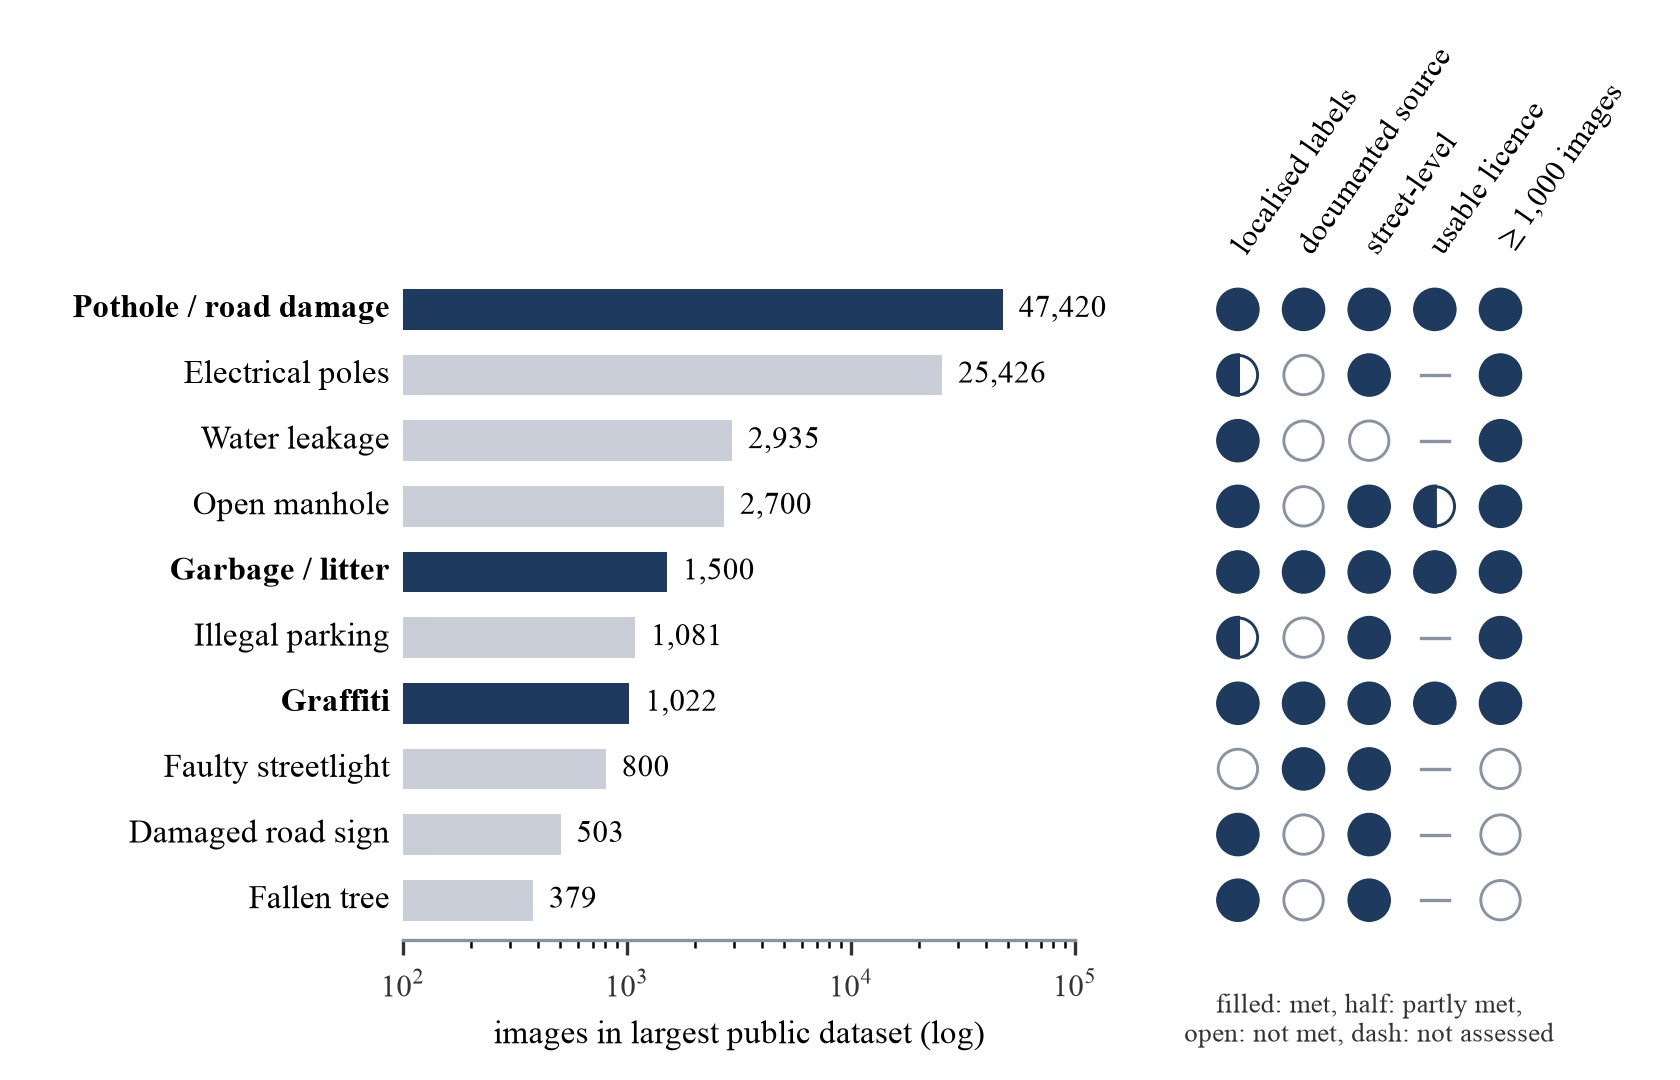
\includegraphics[width=0.96\columnwidth]{figs/fig04.jpg}
\caption{Screening of ten candidate categories against Eq.~(\ref{eq:e1}). Dark bars mark the three categories kept; circles show each criterion met, partly met or not met, and a dash marks a licence not assessed because another criterion already fails.}
\label{fig:f4}
\end{figure}

Fig.~\ref{fig:f5} plots every score Eq.~(\ref{eq:urg}) can produce, read from the server's questionnaire definitions. The pothole questionnaire marks two questions as safety-critical, so its weights sum to 7 and $U$ moves in steps of 1/7. Litter and graffiti mark one, so the sum is 6 and the steps are 1/6. Both profiles have reachable scores in all three bands, but the same answers can land in different bands. One safety-critical ``yes'' gives a pothole $2/7=0.29$, just short of Medium, while the same answer for litter gives $2/6=0.33$ and reaches Medium.

\begin{figure}[!tb]
\centering
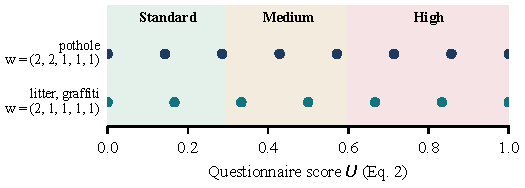
\includegraphics[width=0.96\columnwidth]{figs/fig05.pdf}
\caption{All reachable questionnaire scores for the two weight profiles, with the urgency bands. For a pothole, a single safety-critical ``yes'' scores $2/7=0.29$ and stays in Standard.}
\label{fig:f5}
\end{figure}

\subsection{Per-Category Photo Screening}\label{sec:ai}

For a complaint of category $k$ with photos $x_1,\dots,x_n$ ($n\le3$), the model $f_k$ returns detections $\mathcal{B}_m=f_k(x_m)=\{(b_j,s_j,M_j)\}$ with boxes $b_j$, confidences $s_j$ and, for the litter model, masks $M_j$. After non-maximum suppression the service computes

\begin{align}
s^{*}&=\max_{m}\max_{j} s_j, \label{eq:sstar}\\
\delta&=\max_{m}\frac{\bigl|\bigcup_j M_j^{(m)}\bigr|}{H_m W_m}\quad\text{(litter only)}, \label{eq:delta}\\
r&=\mathbf{1}\left[s^{*}<\tau_k\right], \label{eq:flag}
\end{align}
\noindent where $\tau_k$ is the threshold of category $k$, chosen on validation data by the rule of Eq.~(\ref{eq:tau}), and $r$ is the \texttt{needsReview} flag. If the service fails after two retries, $r=1$. The masked share $\delta$ is stored as descriptive evidence only: it is not a severity measure, since the photo's framing changes it, and it never changes urgency. The model never changes a complaint's stage or urgency. The supervisor sees the annotated photos, $s^{*}$, $\tau_k$ and $r$ next to $u_Q$ and decides (Fig.~\ref{fig:f6}).

The submitted version of this paper raised the suggested urgency one band when $\delta$ exceeded a hand-set threshold $\theta_\delta$, with a single $\tau=0.25$ for every category. Both are removed: two of the three models now predict boxes only, so $\delta$ is not defined for them, and Section~\ref{sec:res} shows that $\tau=0.25$ lets many wrong photos through (\nLitterWrongTwentyfive\,\% of wrong-category litter complaints).

Fig.~\ref{fig:f6} shows the order of events. The questionnaire score is computed when the complaint is filed, and the tracking ID is returned before any inference runs, so the dashed call to the model is the only step that can be slow. The model's detections are reduced to $s^{*}$ and tested once against $\tau_k$. Both branches end in the same triage queue, so a photo the model could not confirm still reaches a person, with a flag, and is never rejected automatically.

\begin{figure}[!tb]
\centering
\resizebox{\columnwidth}{!}{% Fig. 6: photo screening and prioritisation, drawn from backend/services/aiClient.js,
% ai_service/main.py and the supervisor triage screen. Revised: per-category tau_k,
% no model-suggested urgency, delta only as evidence.
\begin{tikzpicture}[
  font=\scriptsize,
  box/.style={draw=markink, rounded corners=1.5pt, align=center, inner sep=3pt, text width=#1, minimum height=8mm},
  box/.default=30mm,
  arr/.style={-{Latex[length=1.6mm]}, markink, line width=0.5pt},
  async/.style={-{Latex[length=1.6mm]}, teal!70!black, dashed, line width=0.6pt},
]
\node[box] (q) at (0,0) {Questionnaire, scored on the server\\$U$, $u_Q$ (Eq.~\ref{eq:urg})};
\node[box] (save) at (4.4,0) {Code checked, consent recorded,\\complaint saved and published,\\tracking ID returned};
\draw[arr] (q) -- node[above] {file} (save);
\node[box, fill=teal!8] (model) at (4.4,-2.0) {Model $f_k$ on each photo $x_m$:\\boxes $b_j$, scores $s_j$, masks $M_j$};
\draw[async] (save) -- node[right] {async} (model);
\node[box, fill=teal!8] (ev) at (0,-2.0) {$s^{*}$ (Eq.~\ref{eq:sstar});\\$\delta$ for litter (Eq.~\ref{eq:delta}),\\shown as evidence only};
\draw[arr] (model) -- (ev);
\node[diamond, draw=markink, fill=teal!8, aspect=2.2, inner sep=1pt, font=\scriptsize] (d) at (0,-3.55) {$s^{*}\ge\tau_k$?};
\draw[arr] (ev) -- (d);
\node[box=22mm, draw=red!60!black] (flag) at (-2.4,-4.85) {$r=1$\\\texttt{needsReview}};
\node[box=22mm, draw=green!45!black] (ok) at (2.4,-4.85) {$r=0$\\no flag};
\draw[arr, red!60!black] (d.west) -| node[pos=0.3, below, align=center] {no, or service\\failed} (flag);
\draw[arr, green!45!black] (d.east) -| node[pos=0.25, above] {yes} (ok);
\node[box=86mm, draw=violet!70!black, fill=violet!6] (tri) at (0.6,-6.25)
  {Supervisor triage: photos with annotations, $u_Q$, $s^{*}$, $\tau_k$, flag $r$\\
   $\Rightarrow$ accept or reject with remarks (a human decision, Eq.~\ref{eq:fsm}); urgency stays $u_Q$};
\draw[arr] (flag) -- (flag |- tri.north);
\draw[arr] (ok) -- (ok |- tri.north);
\draw[arr, dotted, markline] (q.west) -- (-4.1,0 |- q.west) |- node[pos=0.25, left] {$u_Q$} (tri.west);
\end{tikzpicture}
}
\caption{Photo screening and triage. The model's result can only set the review flag $r$; the supervisor decides, and urgency stays the questionnaire band $u_Q$.}
\label{fig:f6}
\end{figure}

\subsection{Auditable Workflow}\label{sec:wf}

The workflow is a deterministic finite-state machine $\mathcal{M}=(S,A,\Delta,s_0,F)$ (Fig.~\ref{fig:f8}) with

\begin{align*}
S&=\{\mathrm{sub},\mathrm{acc},\mathrm{asg},\mathrm{wip},\mathrm{prf},\mathrm{cls},\mathrm{rej}\},\\
A&=\{\mathit{accept},\mathit{reject},\mathit{assign},\mathit{start},\mathit{proof},\mathit{close},\mathit{rework}\},
\end{align*}
\noindent start $s_0=\mathrm{sub}$ and terminal set $F=\{\mathrm{cls},\mathrm{rej}\}$. A transition is applied only if its guard holds:

\begin{equation}
\Delta(s,a)\ \text{is defined} \iff s\in\mathcal{S}_a \wedge \rho(\text{actor})\in\mathcal{R}_a \wedge g_a(c),
\label{eq:fsm}
\end{equation}
\noindent where $\mathcal{S}_a$ and $\mathcal{R}_a$ are the allowed source stages and roles \cite{b49}, and the guard $g_a$ checks remarks ($\ge$10 characters), the ward and leave status of the assignee, and the proof photos. Each transition appends (stage, actor, remarks, $t$) to the history, and \textit{close} emails a PDF receipt. Two staff members acting on the same complaint at the same moment cannot both succeed: the complaint carries a version number, and the slower write fails with 409 instead of overwriting the first. The public sees $\varphi(s)\in\{$Pending, In Progress, Resolved, Rejected$\}$.

Fig.~\ref{fig:f8} shows every path a complaint can take. The main path runs through five transitions from submitted to closed, and Eq.~(\ref{eq:fsm}) guards each one. Rejection is possible only from the submitted stage. After acceptance the only terminal stage left is closed, and reaching it requires proof. If the supervisor finds the proof inadequate, the dashed rework arrow returns the task to assigned, and the loop on assigned lets the supervisor hand it to another worker without changing the stage. The fill colours give the public status. A citizen sees In Progress for all four middle stages, so internal handoffs do not appear on the tracker.

\begin{figure*}[!t]
\centering
\resizebox{0.98\textwidth}{!}{% Fig. 7: physical data model, drawn from backend/models/*.js (eight collections).
% Revised: aiAnalysis fields, consent time, hash-chained access log, export quota,
% unusable password marker; open manhole removed (|C| = 3).
\begin{tikzpicture}[
  font=\tiny,
  ent/.style={draw=#1, line width=0.6pt, rounded corners=1pt, align=left, inner sep=2.5pt, anchor=north west,
              text width=56mm},
  head/.style={fill=#1, text=white, font=\scriptsize\bfseries, anchor=south west, inner sep=2.5pt, text width=56mm},
  rel/.style={markink, line width=0.5pt},
  card/.style={font=\tiny, fill=white, inner sep=0.5pt},
]
% \entity{name}{colour}{position of the body's north-west corner}{body}
\newcommand{\entity}[4]{%
  \node[ent=#2] (#1) at (#3) {#4};
  \node[head=#2] (#1h) at (#1.north west) {#1};}
\entity{Complaint}{markink}{0,0}{%
\textbf{PK} \_id; \textbf{UK} trackingId; \textbf{FK} citizenId $\to$ User\\
title, description, location (identifiers removed)\\
category $\in\mathcal{C}$ ($|\mathcal{C}|=3$), ward\\
answers, urgency score $U$, urgency band $u_Q$\\
stage $\in S$, public status $\varphi(s)$\\
\textbf{FK} assignedTo, assignedBy $\to$ User\\
images[$\le$3], completionImages[$\le$3] (metadata removed)\\
publicationConsentAt, closedAt, isPublic, version key\\
$\triangleright$ \emph{aiAnalysis (1:1)}: state, model, $\tau_k$, $s^{*}$, $\delta$ (litter),\\
\quad needsReview $r$, detections, annotated photos\\
$\triangleright$ \emph{statusHistory[ ]}: stage, actor, remarks, $t$ (append only)}
\entity{Otp}{markline}{$(Complaint.south west)+(0,-0.75)$}{%
email; code hash; attempts $\le$ 5; single use\\
\textbf{TTL} 5 min; matched by email, no stored reference}
\entity{User}{teal!70!black}{6.75,0}{%
\textbf{PK} \_id; \textbf{UK} email; name, phone\\
role (5 account roles), isActive (deactivate only)\\
password: bcrypt (cost 12), or an unusable marker\\
inviteToken (SHA-256, 72 h), mustSetPassword\\
$\triangleright$ \emph{researcher}: scope $\sigma$, granted $t_g$, expires $t_e$\\
$\triangleright$ \emph{employee}: code (\textbf{UK}), ward, supervisor}
\entity{LeaveRequest}{orange!70!black}{$(User.south west)+(0,-0.75)$}{%
\textbf{FK} employeeId, decidedBy $\to$ User\\
fromDate, toDate, reason, status}
\entity{AttendanceRecord}{orange!70!black}{$(LeaveRequest.south west)+(0,-0.75)$}{%
\textbf{UK} (employeeId, date); check-in, check-out}
\entity{ResearchApplication}{violet!70!black}{13.5,0}{%
\textbf{PK} \_id; email, purpose ($\ge$100 characters)\\
requestedDays (1--180), status\\
\textbf{FK} reviewedBy, createdUserId $\to$ User}
\entity{ResearchAccessLog}{violet!70!black}{$(ResearchApplication.south west)+(0,-0.75)$}{%
\textbf{FK} researcherId $\to$ User; action, filters, recordCount\\
\textbf{UK} seq; prevHash, hash (append-only chain)}
\entity{ExportQuota}{violet!70!black}{$(ResearchAccessLog.south west)+(0,-0.75)$}{%
\textbf{UK} (researcherId, UTC day); used $\le$ 5; \textbf{TTL} 3 days}
% relationships
\draw[rel] ([yshift=-3mm]Complaint.north east) -- node[card, above, pos=0.12] {0..*} node[card, above, pos=0.88] {1}
  node[card, below, midway] {files} ([yshift=-3mm]Complaint.north east -| User.west);
\draw[rel] ([yshift=-11mm]Complaint.north east) -- node[card, above, pos=0.12] {0..*} node[card, above, pos=0.88] {0..1}
  node[card, below, midway] {assigned} ([yshift=-11mm]Complaint.north east -| User.west);
\draw[rel] ([yshift=-3mm]User.north east) -- node[card, above, pos=0.12] {0..1} node[card, above, pos=0.88] {0..1}
  ([yshift=-3mm]User.north east -| ResearchApplication.west);
\draw[rel] ([yshift=-11mm]User.north east) -- ++(0.35,0) |- node[card, above, pos=0.88] {0..*} (ResearchAccessLog.west);
\draw[rel] ([yshift=-11mm]User.north east) -- ++(0.35,0) |- node[card, above, pos=0.88] {0..*} (ExportQuota.west);
\draw[rel] ([xshift=-12mm]User.south) -- node[card, right, pos=0.6] {0..*} ([xshift=-12mm]User.south |- LeaveRequesth.north);
\draw[rel] (User.south west) ++(-0.2,0.3) -- ++(-0.25,0) |- node[card, above, pos=0.9] {0..*} (AttendanceRecord.west);
\end{tikzpicture}
}
\caption{Physical data model (MongoDB, Mongoose schemas): eight collections. PK, FK, UK and TTL mark primary keys, references, unique and expiry indexes; rows marked $\triangleright$ begin embedded sub-documents. The research access log is append-only and hash-chained.}
\label{fig:f7}
\end{figure*}

\begin{figure}[!tb]
\centering
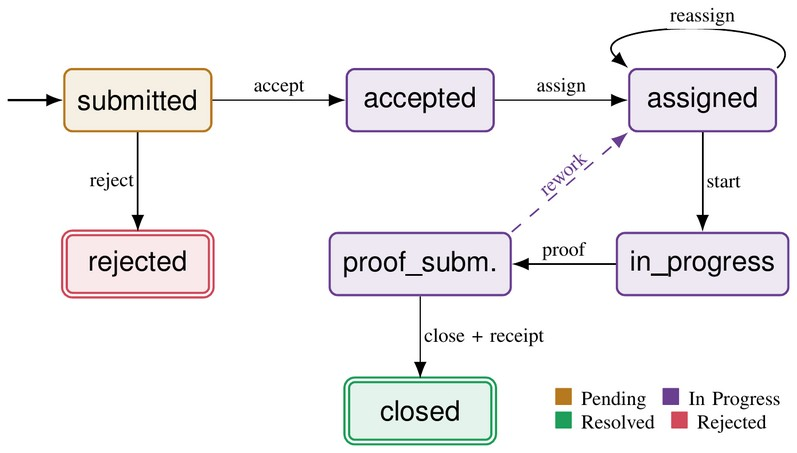
\includegraphics[width=0.79\columnwidth]{figs/fig08.jpg}
\caption{Server-enforced complaint lifecycle (Eq.~\ref{eq:fsm}). Fill colour gives the public status $\varphi(s)$; double borders mark terminal stages.}
\label{fig:f8}
\end{figure}

\subsection{Privacy Analysis}\label{sec:priv}

This subsection states what the system protects, from whom, and how well, measured where possible. Table~\ref{tab:t4} lists what each audience receives, and Table~\ref{tab:t6} maps each adversary to its controls.

\subsubsection{Assets}
The assets are the citizen's identity and contact data (name, email, phone), the photos and their metadata, the free text, and the location and time of filing. Staff identities and the research access records are also personal data.

\subsubsection{Adversaries}
We consider (a) any member of the public using the registry and the tracker; (b) an approved researcher; (c) two or more researchers who combine their exports; (d) an insider with administrator rights; and (e) an outside attacker who obtains a copy of the database.

\begin{table}[!tb]
\caption{Disclosure of one complaint record by audience}
\label{tab:t4}
\centering
\scriptsize
\setlength{\tabcolsep}{1.4pt}
\begin{tabular}{@{}lcccccc@{}}
\toprule
Attribute & Admin & Staff & Registry & Tracker & Res. rec. & Res. agg.\\
\midrule
Citizen identity & \yes & \no & \no & \no & \no & \no\\
Staff identity & \yes & \yes & \no & \no & \no & \no\\
Record ID & \yes & \yes & \yes & \yes & \part & \no\\
Title, description, photos & \yes & \yes & \yes & \yes & \no & \no\\
Street location & \yes & \yes & \yes & \yes & \no & \no\\
Ward & \yes & \yes & \yes & \yes & \yes & \yes\\
Category, urgency, status & \yes & \yes & \yes & \yes & \yes & \part\\
Timestamps & \yes & \yes & \yes & \yes & \part & \part\\
History with remarks & \yes & \yes & \part & \part & \no & \no\\
\bottomrule
\multicolumn{7}{@{}p{\columnwidth}@{}}{\scriptsize \part~transformed: per-researcher HMAC ID, quarter filed, staff shown by role only, or aggregated by month with counts below 5 hidden. Research records in classes smaller than $k=5$ are withheld.}
\end{tabular}
\end{table}

\subsubsection{Controls}
For the public (a), the registry and the tracker are built from an allow-list of fields, so a field added to the database later is not published by accident. Photos are re-encoded without metadata, and phone numbers, email addresses, Aadhaar and PAN numbers and vehicle plates are removed from the published text. Before the code is sent, the citizen must agree to publication of the title, description, photos, street location and ward; the server refuses a complaint without this consent and stores its time. Staff appear on the tracker by role only.

For a researcher (b), the server applies the fixed projection
\begin{equation}
\pi_\rho(c)=\bigl(h_{\kappa_\rho}(c.\mathit{id}),\,k,\,u_Q,\,\varphi,\,\mathit{ward},\,\lfloor t_f\rfloor_{q}\bigr),
\label{eq:proj}
\end{equation}
where $\lfloor\cdot\rfloor_q$ truncates the filing time to the calendar quarter and $\rho$ is the researcher. No closing date or resolution time is released at record level; resolution times are available only as aggregates. Records are then grouped by all released fields except the ID, and every group with fewer than $k=\nChiK$ members is withheld ($k$-anonymity \cite{b37}). Date filters are widened to whole quarters, so a narrow filter cannot isolate a group, and the number of withheld records is not returned, since a researcher could otherwise read a small group's size from it. Aggregates are by month, and any cell, or any resolved or unresolved part of a cell, below 5 is hidden. Access also needs a scope $\sigma$ and an expiry $t_e\le t_g+180$ days, and a request $q$ is served only if
\begin{equation}
\begin{aligned}
&t_q<t_e\ \wedge\ \bigl(\mathrm{rows}(q)\Rightarrow\sigma=\mathrm{records}\bigr)\\
&\wedge\ n_{\mathrm{exp}}(d)\le5\ \wedge\ |q|\le5000,
\end{aligned}
\label{eq:access}
\end{equation}
where $n_{\mathrm{exp}}(d)$ counts the researcher's exports on UTC day $d$ with one atomic database update. Every request is logged (Fig.~\ref{fig:f9}).

For colluding researchers (c), record IDs are keyed per researcher:
\begin{equation}
\begin{aligned}
\kappa_\rho&=\mathrm{HMAC\text{-}SHA256}(\kappa,\rho),\\
h_{\kappa_\rho}(x)&=\mathrm{trunc}_{48}\bigl(\mathrm{HMAC\text{-}SHA256}(\kappa_\rho,x)\bigr),
\end{aligned}
\label{eq:hmac}
\end{equation}
so two exports of the same complaint carry different IDs and cannot be joined on the ID. The research key $\kappa$ is a separate server secret of at least 32 bytes that must differ from the login token secret; the server refuses to start otherwise. Rotating $\kappa$ changes every ID, so a deployment should announce a rotation to researchers in advance.

For an insider (d), staff accounts are only ever deactivated, so history entries keep a valid actor, and the research access log is append-only and hash-chained \cite{b50,b52}: each row stores the SHA-256 of the previous row's hash and its own canonical content, under a unique sequence number. A verifier reports the first broken link. An administrator who rewrites the whole chain is detected only against a head hash published earlier, which is why the current head hash is published in the public statistics. For an outside attacker with a database copy (e), passwords are hashed with bcrypt, one-time codes are stored as hashes, allow five attempts and expire after five minutes, and the HMAC and token secrets are kept out of the database.

\begin{table}[!tb]
\caption{Adversaries and controls}
\label{tab:t6}
\centering
\footnotesize
\setlength{\tabcolsep}{3pt}
\begin{tabular}{@{}p{1.6cm}p{5.5cm}@{}}
\toprule
Adversary & Controls\\
\midrule
(a) Public & Field allow-list; metadata removed from photos; identifiers removed from text; publication consent; staff by role only\\
(b) Researcher & Projection $\pi_\rho$ (Eq.~\ref{eq:proj}); quarter-level dates; $k=5$ withholding; small cells hidden; scope, expiry, quotas (Eq.~\ref{eq:access}); every request logged\\
(c) Colluding researchers & Per-researcher keys $\kappa_\rho$ (Eq.~\ref{eq:hmac})\\
(d) Administrator & Hash-chained access log with a published head hash; deactivate-only accounts\\
(e) Database copy & bcrypt passwords; hashed, single-use codes; secrets outside the database\\
\bottomrule
\end{tabular}
\end{table}

\subsubsection{Pseudonymisation, not anonymisation}
The HMAC IDs are pseudonyms. The research records are therefore pseudonymised personal data in the sense of GDPR Art.~4(5) and Recital~26 \cite{b47,b46} and must be handled as personal data; the submitted version called them anonymised, which was wrong.

\subsubsection{Measured linkage risk}
UrbanFix has no real complaints, so we measured the risk of each candidate release on public data with the same fields: the City of Chicago 311 service requests of 2024 for potholes, fly dumping (litter) and graffiti, \nChiRows{} requests in \nChiWards{} wards after removing \nChiDuplicates{} duplicates. Chicago releases no urgency, so every variant was also measured with a simulated three-level urgency as a worst case. Besides the whole city, we drew \nChiDraws{} samples of \nChiSampleWards{} wards with \nChiSmall{} requests a year, the size of a small deployment, and \nChiMedium{} requests. The adversary knows the category, ward and day filed of one request, as a neighbour who saw it filed would; they \emph{single out} the request when exactly one released record matches, and \emph{learn its outcome} when all matching records share one status and resolution value.

The rule for choosing the release was fixed before the results were seen: the finest of variants C to H whose median withheld share at $k=5$ in the small system, with urgency, is at most 10\,\%; otherwise the variant that withholds least. Table~\ref{tab:t7} gives the results. In the submitted projection (A), \nChiCityKOneA\,\% of the city's records are unique on Chicago's own fields (\nChiCityKOneUrgA\,\% with the simulated urgency, Table~\ref{tab:t7}), and in the small system the adversary singles out \nChiSmallSingledA\,\% of requests. No variant meets the 10\,\% rule. The released variant (H, quarter filed and no resolution time) withholds \nChiSmallWithUrgencyHWithheld\,\% (\nChiHWithheldLo--\nChiHWithheldHi) of records in the small system with urgency, \nChiSmallWithoutUrgencyHWithheld\,\% without it, \nChiMediumWithUrgencyHWithheld\,\% at \nChiMedium{} requests and \nChiCityWithUrgencyHWithheld\,\% across the city. After withholding, the adversary singles out no request (\nChiAfterMax\,\%) in any variant, population or draw. The cost is utility: in a city of the small size, about a third of records are withheld from record-level research, while aggregates lose only cells below five. $k$-anonymity does not stop the second attack: in variant H the adversary still learns the status of \nChiSmallLearnsAfterH\,\% of requests, because most groups share one status ($l$-diversity fails \cite{b41}). For monthly aggregates by ward and category, \nChiCellsSmall\,\% of non-empty cells in the small system and \nChiCellsCity\,\% across the city hold 1 to 4 complaints, which is why such cells are hidden.

\begin{table*}[!t]
\caption{Linkage risk of candidate research releases, Chicago 311 (2024), with simulated urgency. Small system: \nChiSampleWards{} wards, \nChiSmall{} requests, median (5th--95th percentile) over \nChiDraws{} draws. All values in \%.}
\label{tab:t7}
\centering
\footnotesize
\setlength{\tabcolsep}{6pt}
\begin{tabular}{@{}clcccc@{}}
\toprule
& Variant & City & Small: & Small: & Small, after\\
& & $k{=}1$ & withheld & singled & $k{=}5$: learns\\
& & & at $k{=}5$ & out & outcome\\
\midrule
\tablebody{generated/tab_linkage.tex}
\bottomrule
\end{tabular}
\end{table*}

These numbers must be read next to the public registry. The registry shows each complaint's category, ward, street location and exact filing and closing times, without the filer's identity, because public accountability is its purpose; Chicago's own open 311 data does the same. The same adversary therefore singles out a registry entry at least as often as in variant A. The research records add nothing the registry does not already show, and $k=5$ on the research tier is defence in depth: it keeps the research release safe on its own if a municipality restricts or turns off the registry, and it covers bulk, machine-readable exports that leave the system. Minimum cell sizes protect each table, not differences between tables from different filters; formal protection of aggregates would need differential privacy \cite{b42}, which we leave to future work.

\subsubsection{Residual risks}
The main remaining risks are in the registry content: names in free text (the redaction removes patterns such as phone numbers, not names), faces and number plates in photos (no blurring is applied), the street location itself, and very small wards. An adversary who already knows the street location learns nothing new from the research data, but can read the status from the registry, which is public by design.

\subsubsection{Law}
India's Digital Personal Data Protection Act, 2023 \cite{b57} requires notice and consent for processing personal data, limits use to the stated purpose, and requires reasonable security safeguards. Section 17(2)(b) exempts processing for research, archiving or statistical purposes if the data is not used to take any decision specific to the person and the processing follows prescribed standards, which Rule~16 and the Second Schedule of the Digital Personal Data Protection Rules, 2025 set out. The Rules, notified on 14 November 2025, phase in most obligations over eighteen months \cite{b58}. The GDPR \cite{b47} treats pseudonymised data as personal data and names pseudonymisation as a safeguard for research. UrbanFix's notice, consent step, purpose statement for researchers and safeguards are designed with these texts in mind; whether a particular deployment complies is a question for the municipality and its legal advisers, and we make no claim about it.

\begin{figure}[!tb]
\centering
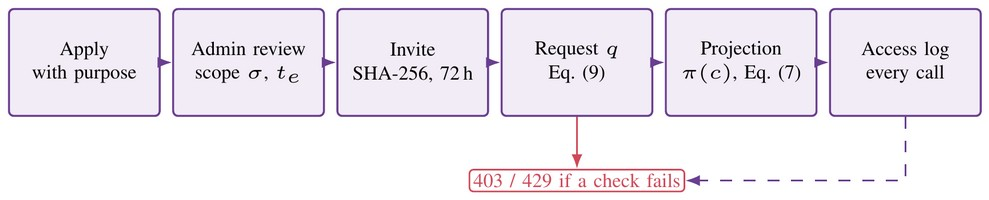
\includegraphics[width=0.99\columnwidth]{figs/fig09.jpg}
\caption{Research access chain. Expiry, scope and quotas are checked on every request (Eq.~\ref{eq:access}), only the projection of Eq.~(\ref{eq:proj}) is returned, and every request is logged.}
\label{fig:f9}
\end{figure}

Fig.~\ref{fig:f9} follows a researcher from application to data. The first three steps happen once. The applicant states a purpose, an administrator sets the scope $\sigma$ and the expiry $t_e$, and the invitation link is stored only as a SHA-256 hash and lapses after 72 hours. The last three steps repeat on every request. The server checks Eq.~(\ref{eq:access}) and answers 403 or 429 if any part fails. A request that passes receives only $k$-anonymised projections, and the request is written to the access log.

\subsection{Data Model}

One User collection holds all five account roles, and Complaint embeds its history and AI analysis (Fig.~\ref{fig:f7}). Every relationship ends at User. A complaint points to users in three ways: the citizen who filed it, the worker it is assigned to, and the actor of each history event. A user has at most one research application and any number of access-log entries, export counters, leave requests and attendance records; unique indexes allow one attendance record per employee per day and one export counter per researcher per day. Otp is matched by email, not by a stored reference, and its TTL index removes each code five minutes after it is issued. A citizen who only files gets an account with an unusable random password marker rather than a bcrypt hash; Section~\ref{sec:val} explains why.

\section{Implementation and Experimental Setup}\label{sec:impl}

The stack is Expo 57, Node.js with Express and Mongoose, and FastAPI with Ultralytics 8.4 \cite{b11}. All code, tests, split lists, result files and the scripts that write every table and figure in this paper are public (see Code and Data Availability).

\subsection{Datasets and Splits}

Table~\ref{tab:t5} lists the datasets. The submitted version used the splits supplied with each dataset. Because several datasets contain edited copies of the same photo, we measured those splits: in the open manhole set, \nOldManholeLeak{} of \nOldManholeVal{} validation images shared a source photo with training, and \nOldManholeCopies{} were augmented copies. The new splits are grouped by source photo. File-name stems and near-duplicate image hashes (a 64-bit difference hash within \nHammingSixtyfour{} bits, confirmed by a 256-bit hash within \nHammingTwofivesix{} bits, mirror images included) form groups, groups are split 70/15/15 with seed 0, and validation, test and external sets keep one image per group. After splitting, \nSplitSharedGroups{} groups, near-duplicate pairs or file stems are shared across splits. For potholes, each country of RDD2022 is split separately, so each has its own test set. The model trained on Japan, the Czech Republic and China only (split \nPotholeNoIndiaSplit) is also tested on all \nExtIndiaAll{} Indian images, and on the \nExtIndiaTest{} Indian test images of the deployed split, to measure the geographic gap.

\begin{table*}[!t]
\caption{Datasets, provenance and splits per category. Splits are grouped by source photo; validation, test and external sets hold one image per source photo. All three licences allow redistribution with attribution.}
\label{tab:t5}
\centering
\footnotesize
\setlength{\tabcolsep}{3pt}
\begin{tabular}{@{}lp{3.2cm}lp{4.2cm}ccp{2.6cm}c@{}}
\toprule
Category & Dataset & Licence & Collector and capture & Labels & Train/val/test & External test (images) & Model\\
\midrule
Pothole & RDD2022, class D40 \cite{b15}; Japan, Czech Rep., China, India$^{e}$ & CC BY 4.0 & Named research team; smartphone and dashboard cameras on public roads; figshare doi:10.6084/m9.figshare.21431547 & boxes & \nPotholeSplit & Roboflow \cite{b16} (\nExtRoboflow)$^{a}$ & v8n\\
Litter & TACO, official annotations \cite{b17} & CC BY 4.0 & Named authors and volunteers; photos of litter in woods, roads and beaches; Zenodo doi:10.5281/zenodo.3587843 & masks$^{b}$ & \nLitterSplit & TACO unofficial (\nExtTacoUnofficial)$^{c}$ & v8n-seg\\
Graffiti & STORM graffiti/tagging \cite{b19} & CC BY 4.0 & Named authors; smartphone photos in Athens via a crowdsensing app; Zenodo doi:10.5281/zenodo.3238357 & boxes & \nGraffitiSplit$^{d}$ & none found & v8n\\
\bottomrule
\multicolumn{8}{@{}p{\textwidth}@{}}{\scriptsize $^{a}$Uploader anonymous, image sources not stated: used for testing only; the training set held 3 augmented copies of each of 240 photos. $^{b}$60 TACO classes merged into one; 1,428 of 1,500 images still available. $^{c}$Public submissions not reviewed by the TACO authors; only the TACO-hosted images marked CC. $^{d}$Test is the official STORM test split. In \nStormBlack{} of the \nStormTotal{} published STORM photos (\nStormBlackTest{} of the \nStormTest{} test photos) the lower part of the image is black. $^{e}$The United States subset consists of Google Street View images, which the CC BY licence cannot cover, and is excluded; a variant trained without Indian photos is tested on all \nExtIndiaAll{} of them to measure the geographic gap.}
\end{tabular}
\end{table*}

\subsection{Training}

Each model is fine-tuned from COCO-pretrained Ultralytics weights at $\nImgSize\times\nImgSize$, batch \nBatch, with the default optimiser and augmentation, for at most \nMaxEpochs{} epochs with early stopping after \nPatience{} epochs without improvement; the checkpoint is chosen on the validation set only. The epoch cap was set by our compute budget (one laptop and a free cloud GPU) and is the same for every model compared. Each number comes from one training run with seed 0; the confidence intervals cover sampling of the test images, not variation between training runs.

\subsection{Metrics}

We report precision $P=TP/(TP+FP)$, recall $R=TP/(TP+FN)$ and the average precision
\begin{equation}
\mathrm{AP}=\int_{0}^{1} p(r)\,dr,
\label{eq:ap}
\end{equation}
\noindent computed as in PASCAL VOC \cite{b54} and COCO \cite{b55}: mAP50 at IoU 0.5 and mAP50--95 averaged over IoU 0.50 to 0.95, on the held-out test split. Intervals are 95\,\% bootstrap percentile intervals over test images with \nBootstrap{} resamples \cite{b59}; rates have Wilson intervals \cite{b60}. CPU latency is the mean time per image over 40 test images, one image at a time with PyTorch's default threading, on an idle Apple M5 laptop.

\subsection{Complaint-Level Screening}

The model's job is to flag complaints, so we evaluate complaints, not only images. A synthetic complaint is 1, 2 or 3 photos drawn uniformly (seed 0) from one set, each photo used once, and it is flagged when $s^{*}<\tau_k$ (Eq.~\ref{eq:flag}). Valid complaints are built from test photos that show the defect; wrong-category complaints from the other categories' test photos; unrelated complaints from a seeded sample of COCO 2017 validation photos \cite{b55}, leaving out, for litter, photos with a bottle, cup or wine glass; and for potholes, also road photos from RDD2022 without a pothole. The threshold of each category is chosen on validation data only (the category's validation split, the other categories' validation splits and half of the COCO sample):
\begin{equation}
\tau_k=\max\{\tau\in\{0.05,0.10,\dots,0.90\} : \widehat{\mathrm{FF}}_{\mathrm{val}}(\tau)\le\nMaxFalseFlagRule\,\%\},
\label{eq:tau}
\end{equation}
where $\widehat{\mathrm{FF}}_{\mathrm{val}}$ is the share of valid validation complaints flagged. A false flag costs a supervisor one look, while a false pass lets a wrong photo through unmarked, although supervisors still see every complaint; the rule therefore accepts up to one false flag in five valid complaints to pass as few wrong photos as possible. We compare YOLOv8n with YOLO11n \cite{b61} and with RT-DETR-l \cite{b56}, all trained on the same splits with the same budget. Two ablations test design choices of the submitted version: graffiti trained without COCO pretraining, and litter trained on TACO's 28 super-categories instead of one merged class (scored as one class). The model to deploy is YOLOv8n unless another model is better on the test set at no more than 2 to 4 times its CPU latency.

\section{Results and Discussion}\label{sec:res}

\subsection{Detection on the Test Sets}

Table~\ref{tab:t8} gives the deployed models' test results. Box mAP50 is \nPotholeTestMap{} for potholes, \nLitterTestMap{} for litter and \nGraffitiTestMap{} for graffiti. The validation column is not an independent estimate: it chose the checkpoint. The submitted version reported validation scores only, on splits that leaked, so its numbers are not comparable. Inference takes \nCpuMsMin{} to \nCpuMsMax{} ms per photo on the laptop CPU, so no GPU server is needed.

\begin{table*}[!t]
\caption{Deployed models on the held-out test splits (box metrics; mask mAP50 for litter). 95\,\% bootstrap intervals over test images. One training run each (seed 0).}
\label{tab:t8}
\centering
\footnotesize
\setlength{\tabcolsep}{4pt}
\begin{tabular}{@{}lcccccccc@{}}
\toprule
Category & Test images & $P$ & $R$ & mAP50 & mAP50--95 & Mask mAP50 & Val. mAP50 & Best epoch\\
\midrule
\tablebody{generated/tab_detection.tex}
\bottomrule
\end{tabular}
\end{table*}

Fig.~\ref{fig:f11} shows that all three models reached their best validation score at epoch \nPotholeBestEpoch{}, \nLitterBestEpoch{} and \nGraffitiBestEpoch{} of \nMaxEpochs{}, so they were still improving when the cap stopped them. The cap may understate YOLOv8n against models that converge faster; we state this as a limitation rather than tune the budget per model.

\begin{figure}[!tb]
\centering
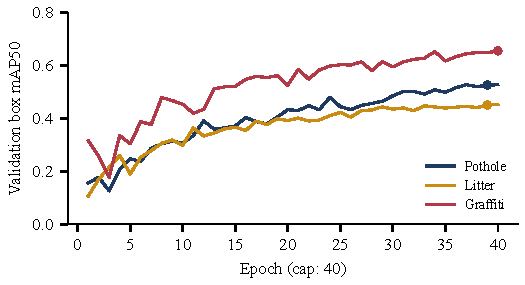
\includegraphics[width=\columnwidth]{figs/fig_curves.pdf}
\caption{Validation box mAP50 per epoch for the deployed models; dots mark the chosen checkpoint. Training and validation data only.}
\label{fig:f11}
\end{figure}

\subsection{Baselines and Ablations}

Table~\ref{tab:t9} compares the detectors. YOLO11n is not better than YOLOv8n for any category at the same latency. RT-DETR-l has the highest point estimate for every category, most clearly for graffiti (\nGraffitiRtdetrLMap{} against \nGraffitiYolovEightnMap), although its interval overlaps YOLOv8n's in every category, so no difference is established at this test-set size; it takes about \nGraffitiRtdetrLCpuMs{} ms per photo on the CPU against \nGraffitiYolovEightnCpuMs{} ms, and its weights are \nGraffitiRtdetrLMb{} MB against \nGraffitiYolovEightnMb{} MB. That is far beyond the rule's 2 to 4 times, so YOLOv8n is deployed; a municipality with a GPU server could choose RT-DETR-l for graffiti. For litter, RT-DETR-l's higher mAP does not carry over to complaints: at its threshold it passes \nLitterRtdetrLUnrelatedPass\,\% of unrelated complaints against \nLitterYolovEightnUnrelatedPass\,\% for YOLOv8n. Both ablations support the submitted design. Without pretraining, graffiti mAP50 falls to \nGraffitiYolovEightnScratchMap{} and unrelated photos pass \nGraffitiYolovEightnScratchUnrelatedPass\,\% of the time; with 28 litter classes, mAP50 is \nLitterYolovEightnSuperMap{} and unrelated photos pass \nLitterYolovEightnSuperUnrelatedPass\,\% of the time.

\begin{table*}[!t]
\caption{Baselines and ablations on the test splits. Rates are shares of synthetic test complaints at each model's own $\tau_k$ (Eq.~\ref{eq:tau}). CPU: mean ms per photo on the same idle laptop.}
\label{tab:t9}
\centering
\footnotesize
\setlength{\tabcolsep}{4pt}
\begin{tabular}{@{}llccccccc@{}}
\toprule
Category & Model & Box mAP50 & $\tau_k$ & Valid & Wrong-category & Unrelated & CPU & Size\\
& & (95\,\% CI) & & flagged (\%) & passed (\%) & passed (\%) & (ms) & (MB)\\
\midrule
\tablebody{generated/tab_baselines.tex}
\bottomrule
\multicolumn{9}{@{}p{0.9\textwidth}@{}}{\scriptsize $^{a}$Pothole models in this block are trained without Indian photos (split \nPotholeNoIndiaSplit) so that all three detectors share one split; the deployed pothole model in Table~\ref{tab:t8} adds India.}
\end{tabular}
\end{table*}

\subsection{Complaint-Level Screening}

Table~\ref{tab:t10} gives the screening rates of the deployed models, and Fig.~\ref{fig:f12} shows how $\tau_k$ was chosen. At the chosen thresholds, \nFlagMin\,\% to \nFlagMax\,\% of valid complaints are flagged, so a supervisor looks again at roughly one valid complaint in four to nine. In exchange, wrong-category photos pass in \nGraffitiWrong\,\% (graffiti) to \nLitterWrong\,\% (litter) of complaints. At the single threshold $\tau=0.25$ of the submitted version, fewer valid complaints are flagged (\nPotholeFlagTwentyfive\,\% for potholes), but \nLitterUnrelatedTwentyfive\,\% of unrelated litter complaints and \nGraffitiUnrelatedTwentyfive\,\% of unrelated graffiti complaints pass: for litter and graffiti that threshold was close to useless as a screen. Litter remains the weakest category for unrelated photos. The pothole model flags \nPotholeFlag\,\% of valid test complaints, more than the \nMaxFalseFlagRule\,\% the rule allowed on validation data, so the rule's bound does not carry over exactly from validation to test.

\begin{table*}[!t]
\caption{Complaint-level screening of the deployed models on synthetic test complaints of 1 to 3 photos, in \% (95\,\% Wilson interval), at the chosen $\tau_k$ and at the submitted $\tau=0.25$.}
\label{tab:t10}
\centering
\footnotesize
\setlength{\tabcolsep}{4pt}
\begin{tabular}{@{}lcccccc@{}}
\toprule
Category & $\tau$ & Valid flagged & Wrong-category passed & Unrelated passed & Road without pothole passed\\
\midrule
\tablebody{generated/tab_screening.tex}
\bottomrule
\end{tabular}
\end{table*}

\begin{figure*}[!t]
\centering
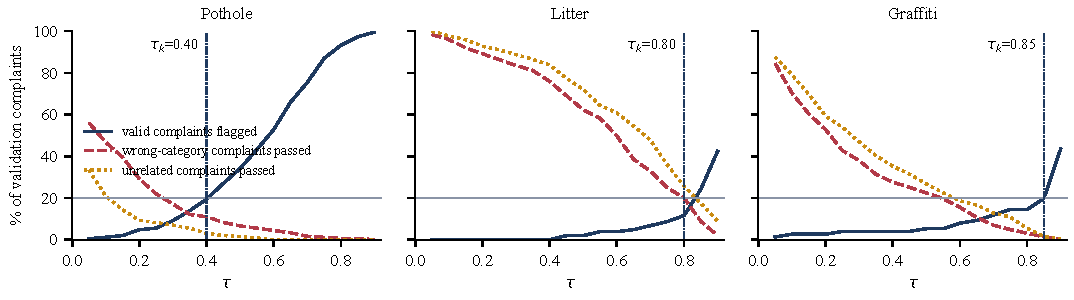
\includegraphics[width=\textwidth]{figs/fig_tau.pdf}
\caption{Choice of $\tau_k$ on validation complaints (Eq.~\ref{eq:tau}): the largest threshold that flags at most 20\,\% of valid complaints (horizontal line). Raising $\tau$ trades more flags on valid complaints for fewer wrong and unrelated photos passing.}
\label{fig:f12}
\end{figure*}

To see what these rates mean for a supervisor, we simulated 100 complaints with an assumed share of invalid ones split evenly between wrong-category and unrelated photos. With 10\,\% invalid, the pothole model flags \nPotholeSimFlagged{} of 100 complaints, of which \nPotholeSimValidFlagged{} are valid, and lets \nPotholeSimInvalidPassed{} invalid complaints through unflagged; for litter the figures are \nLitterSimFlagged, \nLitterSimValidFlagged{} and \nLitterSimInvalidPassed, and for graffiti \nGraffitiSimFlagged, \nGraffitiSimValidFlagged{} and \nGraffitiSimInvalidPassed. This is a simulation with an assumed invalid share, not a measurement of staff decisions; a study of supervisors with and without the model is future work.

Fig.~\ref{fig:f10} shows one example per category, chosen by rule: among the valid test photos that pass $\tau_k$, the one whose $s^{*}$ is the median. Fig.~\ref{fig:f13} shows the errors. The top row of each panel holds the four valid test photos with the lowest $s^{*}$, which the model flags. The bottom row holds the four wrong-category or unrelated photos with the highest $s^{*}$, which pass; the detection that made them pass is drawn in red. COCO photos whose licence does not allow reuse in this paper (non-commercial, no-derivatives or share-alike) are shown as grey tiles with their COCO id. The black lower halves of two graffiti photos are in the published STORM files (Table~\ref{tab:t5}).

\begin{figure*}[!t]
\centering
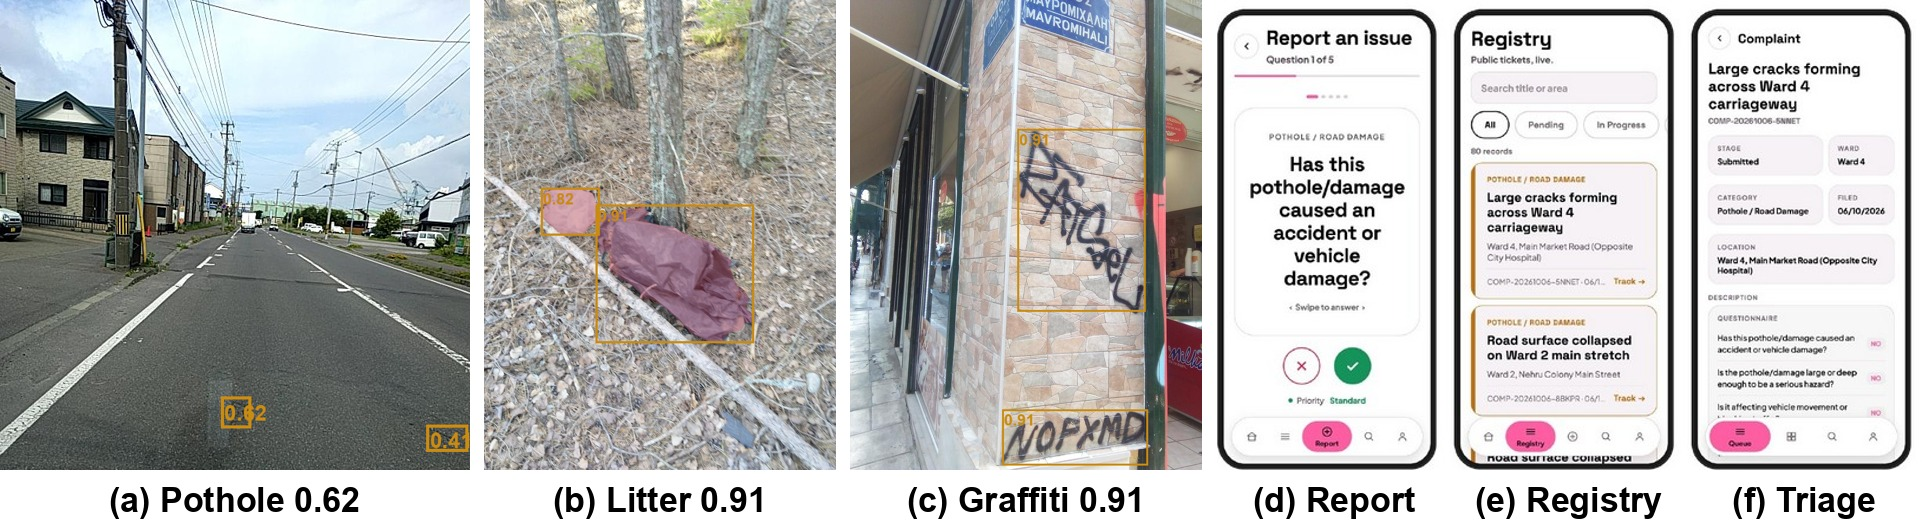
\includegraphics[width=\textwidth]{figs/fig10.jpg}
\caption{(a)--(c) Deployed models on test photos at their $\tau_k$, with $s^{*}$: the photo with the median $s^{*}$ among valid test photos that pass. Boxes and confidences in orange; the litter model also draws masks. (d)--(f) App screens: weighted swipe questionnaire with live urgency, public registry and supervisor triage (seeded demonstration data).}
\label{fig:f10}
\end{figure*}

\begin{figure*}[!p]
\centering
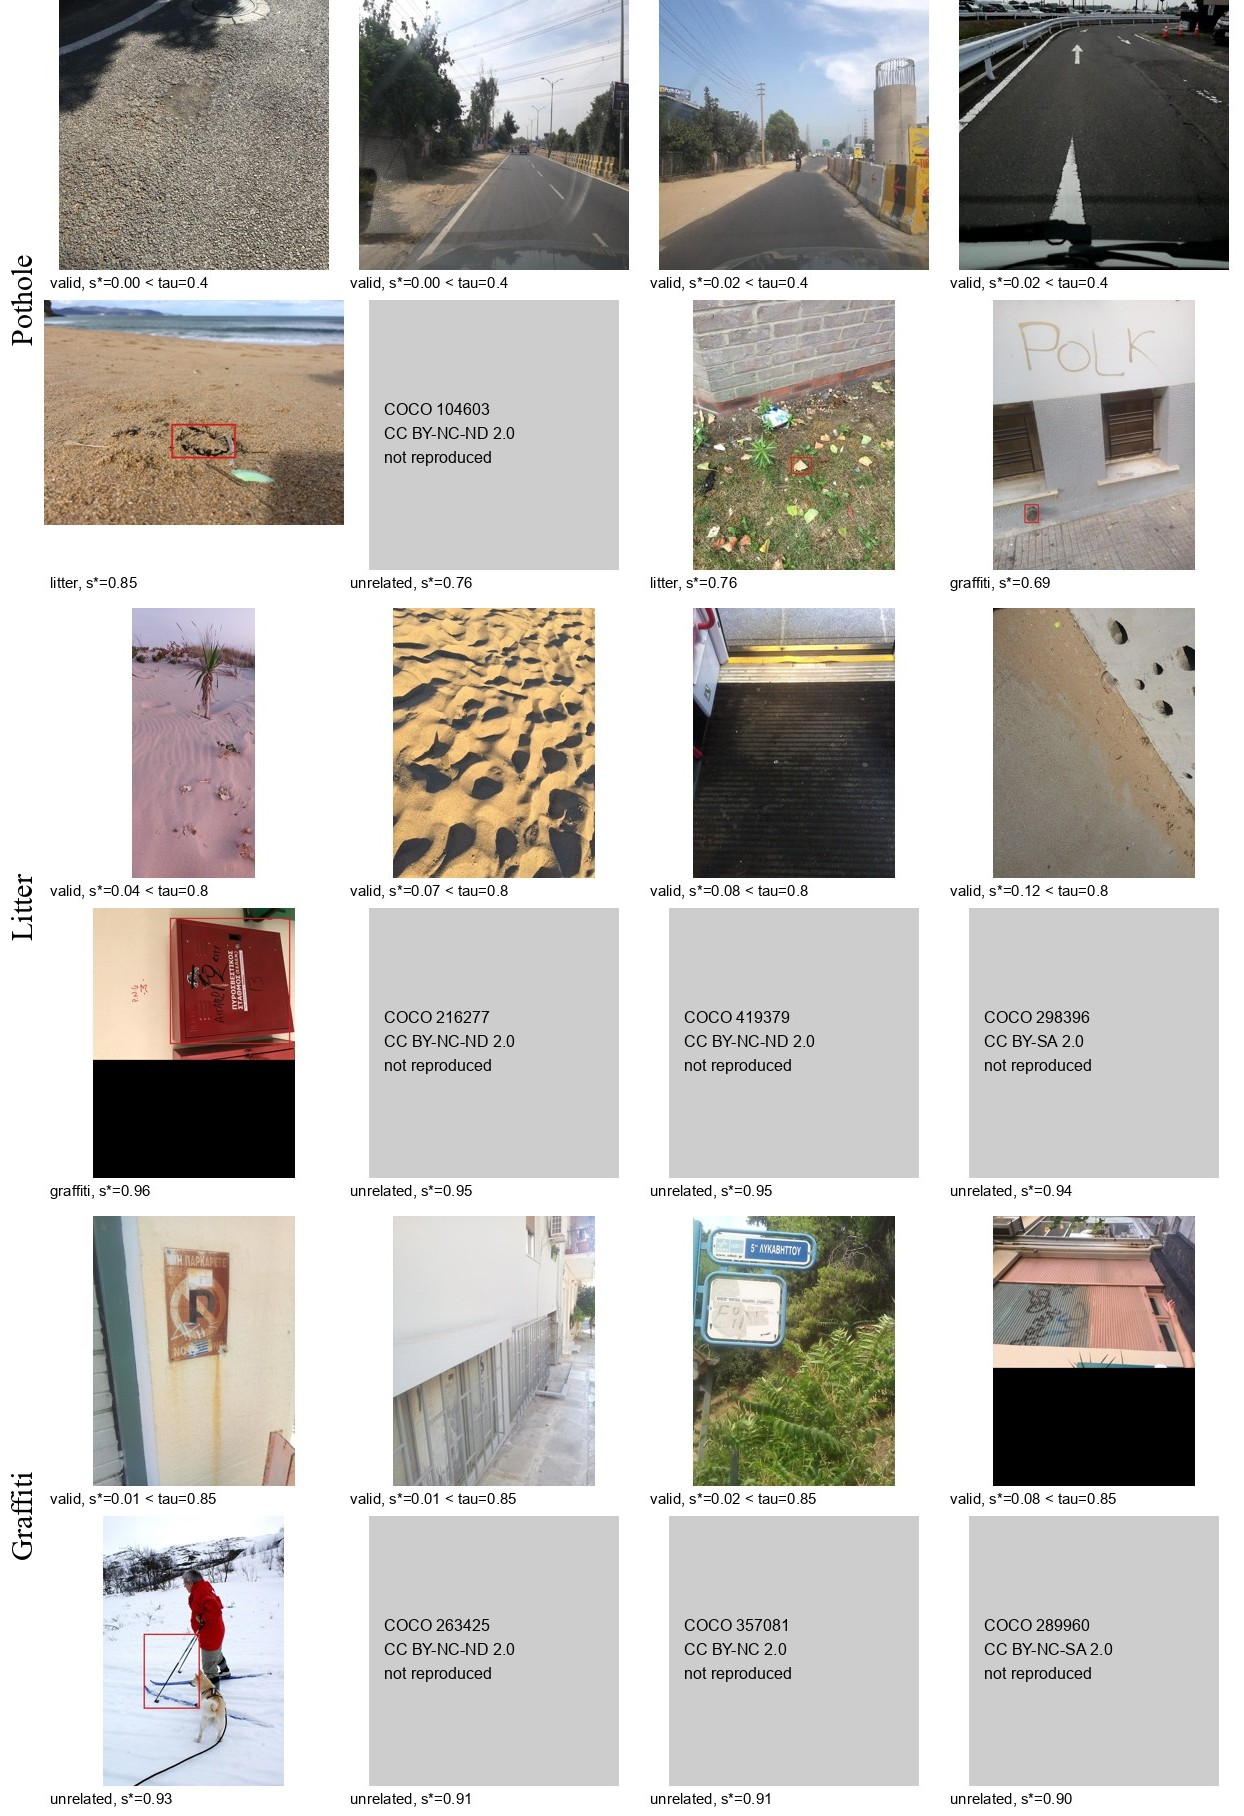
\includegraphics[width=0.82\textwidth]{figs/fig_errors.jpg}
\caption{Error analysis of the deployed models. In each panel, top: the four valid test photos with the lowest $s^{*}$ (flagged at $\tau_k$); bottom: the four wrong-category or unrelated photos with the highest $s^{*}$ (passed), with the passing detection in red. Grey tiles stand for COCO photos whose licence does not allow reproduction here.}
\label{fig:f13}
\end{figure*}

\subsection{Cross-Dataset Tests and the Geographic Gap}

External sets test the models on photos from other sources. On the Roboflow pothole photos, mostly close-ups, box mAP50 is \nRoboflowMapWith{} for the deployed model, and \nRoboflowFlag\,\% of valid complaints are flagged. On TACO's unofficial annotations, taken by other photographers, the litter model reaches \nTacoUnofficialMap{} and flags \nTacoUnofficialFlag\,\% of valid complaints. The pothole result is far below the in-domain test result and the litter result somewhat below it, so a deployment should expect more flags on its own photos.

The largest gap is geographic (Table~\ref{tab:t11}, Fig.~\ref{fig:f14}). The pothole model trained on Japan, the Czech Republic and China reaches box mAP50 \nGeoIndiaMapNo{} on the \nGeoIndiaImages{} Indian test photos and \nGeoIndiaAllMap{} on all \nExtIndiaAll{} Indian photos, against \nGeoJapanMapNo{} on Japanese ones, and it flags \nGeoIndiaFlagNo\,\% (\nGeoIndiaFlagNoLo--\nGeoIndiaFlagNoHi) of valid Indian complaints. RT-DETR-l and YOLO11n trained on the same data reach only \nGeoIndiaRtdetrL{} and \nGeoIndiaYoloOneOnen{} on the Indian test photos, so the gap comes from the training data, not from the detector. Adding Indian photos to training (the deployed model) raises mAP50 on the same Indian test photos to \nGeoIndiaMapWith{} and lowers the share of valid Indian complaints flagged to \nGeoIndiaFlagWith\,\% (\nGeoIndiaFlagWithLo--\nGeoIndiaFlagWithHi), about twice the Japanese rate of \nGeoJapanFlagWith\,\%. The Czech and Chinese test sets are small (\nGeoCzechFlagN{} and \nGeoChinaFlagN{} complaints), and their intervals are too wide to rank.

\begin{table*}[!t]
\caption{Pothole screening by country: box mAP50 (95\,\% CI) and valid complaints flagged (\%, Wilson CI), for the model trained without and with Indian photos, on the same test photos.}
\label{tab:t11}
\centering
\footnotesize
\setlength{\tabcolsep}{6pt}
\begin{tabular}{@{}lccccc@{}}
\toprule
& & \multicolumn{2}{c}{Trained without India} & \multicolumn{2}{c}{With India (deployed)}\\
Country & Img. & mAP50 & Flagged & mAP50 & Flagged\\
\midrule
\tablebody{generated/tab_geography.tex}
\bottomrule
\end{tabular}
\end{table*}

\begin{figure}[!tb]
\centering
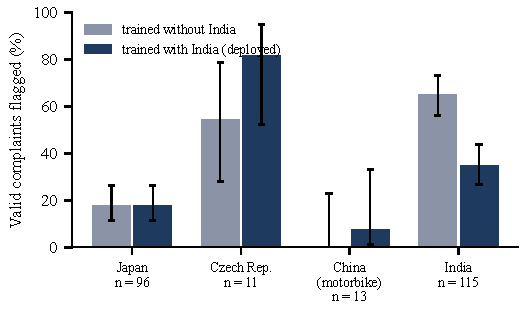
\includegraphics[width=\columnwidth]{figs/fig_geo.pdf}
\caption{Share of valid pothole complaints flagged per country, with 95\,\% Wilson intervals, for the model trained without Indian photos ($\tau=0.50$) and the deployed model trained with them ($\tau=0.40$). $n$: valid test complaints per country.}
\label{fig:f14}
\end{figure}

\subsection{Fairness}\label{sec:fair}

\emph{Who reports.} Studies of 311 and FixMyStreet data find lower reporting in poorer and minority areas \cite{b12,b13,b14}, so complaint counts are a biased guide to need. UrbanFix does not rank wards by complaint counts, and its counts must not be used to allocate resources without correcting for who reports.

\emph{Access.} Filing needs a smartphone, an email address and literacy in the app's language. Account-free filing removes one barrier but not these.

\emph{Which problems can be reported.} Eq.~(\ref{eq:e1}) lets data availability decide which problems citizens can report. Water leakage and streetlights are excluded for lack of usable data, not lack of need.

\emph{Model bias by place.} A flagged complaint waits for a person, so a model that flags Indian photos more often delays Indian complainants. Human review limits the harm, since no complaint is rejected by the model, but it does not remove the delay. Training on Indian photos roughly halved the share of Indian complaints flagged but did not close the gap with Japan (Table~\ref{tab:t11}); fine-tuning on photos from the deploying city is the next step \cite{b48}.

\emph{Monitoring.} The administrator dashboard reports, per ward, the share of model-checked complaints that were flagged and the median days from filing to closure, so a ward whose complaints are flagged more often or closed more slowly becomes visible.

\subsection{System Validation}\label{sec:val}

Table~\ref{tab:t12} lists the automated tests, which run on every push to the public repository. The backend tests start the API with an in-memory MongoDB and exercise it over HTTP; the sixteen API tests of the submitted version are kept, now automated. Beyond them, the tests check that five wrong codes lock a code and that it cannot be reused; that two simultaneous transitions on one complaint and parallel exports beyond the daily quota cannot both succeed; that editing or deleting an access-log row breaks the hash chain at that row; that GPS and camera metadata are gone from served photos and identifiers from published text; that research records in classes under five are withheld and that a day-level filter cannot isolate them; and that a complaint without publication consent is refused. The one skipped test needs the vision service and runs in the continuous-integration job that starts it.

\begin{table}[!tb]
\caption{Automated tests (JUnit reports in the repository). $^{*}$The skipped test needs the running vision service; it runs in the continuous-integration job that starts the service.}
\label{tab:t12}
\centering
\footnotesize
\setlength{\tabcolsep}{3pt}
\begin{tabular}{@{}p{5.4cm}cc@{}}
\toprule
Group & Tests & Passed\\
\midrule
\tablebody{generated/tab_tests.tex}
\bottomrule
\end{tabular}
\end{table}

Table~\ref{tab:t13} gives a load test on one laptop (\nLoadCpu, \nLoadComplaints{} seeded complaints, \nLoadDuration{} s per scenario; the load generator runs on the same machine). At 50 connections every scenario ran without errors. Research records take \nLoadResearchRecordsFiveZerorps{} requests per second, against \nLoadRegistryListFiveZerorps{} for the registry, because each request counts equivalence classes over all matching complaints before releasing any. At 200 connections up to \nLoadRegistryListTwoZeroZeroerrors\,\% of requests failed, because macOS limits the listen backlog to 128 connections; the numbers describe one machine and are not a claim about city-scale capacity. Filing was first limited to \nLoadSubmitBeforeRps{} complaints per second (median \nLoadSubmitBeforePfifty{} ms), because every first-time citizen received a random password hashed with bcrypt at cost 12, which blocked the server's single event loop for each new citizen. Citizens who only file now get an unusable random marker instead, which cannot be used to log in, and filing rose to \nLoadSubmitTwoZerorps{} complaints per second (median \nLoadSubmitTwoZeropfifty{} ms). The vision service does not slow filing, because the model runs after the response.

\begin{table}[!tb]
\caption{Load test (autocannon; latency in ms; p97.5 is reported because autocannon gives it instead of p95). Research records are $k$-anonymised and every request is logged.}
\label{tab:t13}
\centering
\scriptsize
\setlength{\tabcolsep}{2.2pt}
\begin{tabular}{@{}p{2.3cm}cccccc@{}}
\toprule
Scenario & Conn. & Req/s & p50 & p97.5 & p99 & Err.\,\%\\
\midrule
\tablebody{generated/tab_load.tex}
\bottomrule
\end{tabular}
\end{table}

\subsection{Deployment Cost}

The slowest deployed model takes \nCpuMsMax{} ms per photo on the laptop CPU (PyTorch's default threading, one photo at a time), so a complaint of three photos needs about \nCostMsPerComplaint{} ms, and one such machine could screen roughly \nCostPerCoreDay{} complaints a day. CPGRAMS, India's national grievance portal, received at most 26.2 lakh grievances in a year \cite{b3,b4}, about \nCostCpgramsPerDay{} a day, or \nCostCoreShare\,\% of that capacity. Screening is therefore not the cost that matters; staff time for triage is, which the flag rates of Table~\ref{tab:t10} determine. This estimate covers inference only, on our hardware; it is not a field measurement.

\subsection{Demonstration Data}

To exercise the dashboards we seeded 80 complaints over twelve months (Fig.~\ref{fig:f16}): 41 were accepted, 9 rejected and 19 closed, after 8.2 to 9.2 days on average. Each stage holds fewer complaints than the one before because the workflow never skips a stage. With two to nine closed complaints per category and seeded data, the panel shows only that the dashboards compute the measures; no real ward was measured.

\begin{figure}[!tb]
\centering
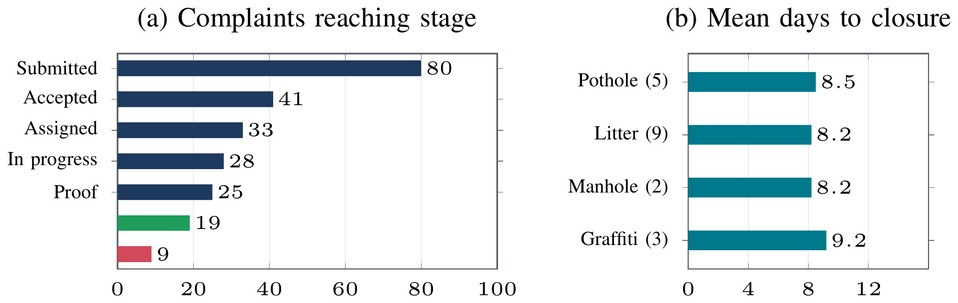
\includegraphics[width=0.96\columnwidth]{figs/fig16.jpg}
\caption{Workflow on the seeded demonstration dataset (n = 80); closed complaints per category in brackets. They exercise the dashboards only; no real ward was measured.}
\label{fig:f16}
\end{figure}

\subsection{Limitations}

UrbanFix has not been deployed: there are no real complaints, and no staff or citizen study, so the effect of the flags on supervisors' decisions and workload is simulated, not measured. The synthetic complaints are built from single dataset photos and may differ from what citizens submit. Each model was trained once (seed 0) with a \nMaxEpochs-epoch cap that stopped all three while they were still improving. Apart from RDD2022's Indian subset, the training photos come from outside India, and graffiti has no external test set. The questionnaire weights were set by hand. The residual privacy risks of Section~\ref{sec:priv} remain: names in free text, faces and plates in photos, and the street location in the registry. The fairness limits of Section~\ref{sec:fair} also remain, and there is no GPS capture or duplicate detection.

\section{Conclusion and Future Work}\label{sec:conc}

UrbanFix takes a civic complaint from the citizen's photo to a recorded repair using open-source software and public data. A per-category model screens the photo and can only flag it for a person, a supervisor triages it, and the server enforces each step before the record is published without the filer's identity. Measured at the level of complaints, the models flag \nFlagMin\,\% to \nFlagMax\,\% of valid complaints at thresholds chosen by a written rule, and the single threshold of the submitted version let most unrelated litter and graffiti photos through. Training on Indian photos roughly halved the share of Indian pothole complaints flagged. Measuring linkage risk on Chicago 311 data showed that the submitted research projection singled out most requests in a small city, and set the quarter-level, $k=5$ release the server now enforces. Next we will run a ward-level pilot with a municipal corporation, fine-tune the models on its photos, study supervisors' decisions with and without the model, fit the questionnaire weights to closed complaints, and add blurring of faces and number plates.

\section*{Code and Data Availability}

The source code (MIT licence), the model weights (AGPL-3.0, as they are fine-tuned from Ultralytics weights), the split lists, the result files, the test reports and the scripts that generate every table and figure of this paper are available at \repoURL{} and archived at \archiveDOI. Dataset images are not redistributed; the repository contains scripts that download them from their publishers (Table~\ref{tab:t5}), and the Chicago 311 extract is fetched from the City of Chicago Data Portal by a script that records its checksum. No real complaint data exists, because the system has not been deployed.

\clearpage
\begin{thebibliography}{00}
\bibitem{b1} Ministry of Road Transport and Highways, Government of India, ``Road Accidents in India,'' annual reports 2018--2022, New Delhi.
\bibitem{b2} Ministry of Road Transport and Highways, written reply on pothole-related road accidents 2020--2024, Lok Sabha, Feb. 2026.
\bibitem{b3} Press Information Bureau, ``Grievance cell,'' Ministry of Personnel, Public Grievances and Pensions, Mar. 16, 2022. [Online]. Available: \url{https://pib.gov.in/PressReleasePage.aspx?PRID=1806610}
\bibitem{b4} Press Information Bureau, ``Disposal rate of grievance redressal mechanism,'' Apr. 2, 2025. [Online]. Available: \url{https://pib.gov.in/PressReleasePage.aspx?PRID=2117810}
\bibitem{b5} Press Information Bureau, ``CPGRAMS portal,'' Feb. 5, 2026. [Online]. Available: \url{https://pib.gov.in/PressReleasePage.aspx?PRID=2223804}
\bibitem{b6} S. K. Kanagapriya and V. Kesika, ``AI-driven anonymous civic intelligence for transparent and efficient municipal governance,'' in \textit{Proc. 7th Int. Conf. Intelligent Communication Technologies and Virtual Mobile Networks (ICICV)}, 2026, pp. 1582--1589, doi: 10.1109/ICICV68925.2026.11554648.
\bibitem{b7} R. Praveen Kumar, P. Sam Benny, Ch. Manideep, G. Sushmitha, and Md. Athfaan, ``Smart City Concern: An AI-driven multimodal civic grievance management system,'' in \textit{Proc. 6th Int. Conf. Trends in Material Science and Inventive Materials (ICTMIM)}, 2026, pp. 1894--1901, doi: 10.1109/ICTMIM68190.2026.11507401.
\bibitem{b8} P. Cholke, A. S. Mishra, V. N. Mehar, M. Chikhale, H. Marathe, and D. Nhalade, ``AI-driven complaint management system: An automated framework for prioritizing, tracking, and resolving public service complaints efficiently,'' in \textit{Proc. Int. Conf. Emerging Smart Computing and Informatics (ESCI)}, 2026, doi: 10.1109/ESCI68015.2026.11493166.
\bibitem{b9} M. Vishwanath, A. M. Vasudha, P. U. Kulkarni, M. K. Prakruthi, and V. V. Murthy, ``AI-driven smart waste management with geofencing and civic accountability,'' in \textit{Proc. 3rd Int. Conf. Emerging Applications of Material Science and Technology (ICEAMST)}, 2025, doi: 10.1109/ICEAMST67459.2025.11336075.
\bibitem{b10} S. Salunkhe, T. Salunke, A. Saware, A. Salvi, A. Patil, and R. Jolhe, ``CivicMate: An AI-driven city grievances,'' in \textit{Proc. 6th Biennial Int. Conf. Nascent Technologies in Engineering (ICNTE)}, 2026, doi: 10.1109/ICNTE66387.2026.11437408.
\bibitem{b11} G. Jocher, A. Chaurasia, and J. Qiu, ``Ultralytics YOLOv8,'' version 8.0.0, 2023. [Online]. Available: \url{https://github.com/ultralytics/ultralytics}
\bibitem{b12} B. Y. Clark, J. L. Brudney, and S.-G. Jang, ``Coproduction of government services and the new information technology: Investigating the distributional biases,'' \textit{Public Admin. Rev.}, vol. 73, no. 5, pp. 687--701, 2013, doi: 10.1111/puar.12092.
\bibitem{b13} B. Pak, A. Chua, and A. Vande Moere, ``FixMyStreet Brussels: Socio-demographic inequality in crowdsourced civic participation,'' \textit{J. Urban Technol.}, vol. 24, no. 2, pp. 65--87, 2017, doi: 10.1080/10630732.2016.1270047.
\bibitem{b14} C. E. Kontokosta and B. Hong, ``Bias in smart city governance: How socio-spatial disparities in 311 complaint behavior impact the fairness of data-driven decisions,'' \textit{Sustain. Cities Soc.}, vol. 64, Art. no. 102503, 2021, doi: 10.1016/j.scs.2020.102503.
\bibitem{b15} D. Arya, H. Maeda, S. K. Ghosh, D. Toshniwal, and Y. Sekimoto, ``RDD2022: A multi-national image dataset for automatic road damage detection,'' \textit{Geosci. Data J.}, 2024, doi: 10.1002/gdj3.260. Data: doi: 10.6084/m9.figshare.21431547, CC BY 4.0.
\bibitem{b16} Roboflow Universe, ``Pothole segmentation YOLOv8 dataset, v1,'' CC BY 4.0. [Online]. Available: \url{https://universe.roboflow.com/farzad/pothole_segmentation_yolov8}
\bibitem{b17} P. F. Proença and P. Simões, ``TACO: Trash annotations in context for litter detection,'' arXiv:2003.06975, 2020. Data: Zenodo, doi: 10.5281/zenodo.3587843, CC BY 4.0.
\bibitem{b19} C. Patrikakis, P. Kasnesis, L. Toumanidis, and A. Tzitamidis, ``STORM graffiti/tagging detection dataset,'' Univ. of West Attica, Zenodo, 2019, doi: 10.5281/zenodo.3238357.
\bibitem{b20} S. Chen, Y. Zhang, B. Song, X. Du, and M. Guizani, ``An intelligent government complaint prediction approach,'' \textit{Big Data Res.}, vol. 30, Art. no. 100336, 2022, doi: 10.1016/j.bdr.2022.100336.
\bibitem{b21} P. M. Javali, K. Naregal, A. Gudnavar, S. Athanikar, and S. Shinde, ``A web-based public grievance redressal system with image and geolocation support,'' in \textit{Proc. Int. Conf. Smart \& Sustainable Technology (INCSST)}, 2025, doi: 10.1109/INCSST64791.2025.11210297.
\bibitem{b22} S. N. Katkar, V. Makadiya, A. Mane, V. Parab, and M. Pingale, ``CivicX: An AI-driven data-centric platform for urban grievance management and intelligent plan approval,'' in \textit{Proc. Int. Conf. Communication, Computing and Emerging Technologies (IC3ET)}, 2026, pp. 631--641, doi: 10.1109/IC3ET64989.2026.11467223.
\bibitem{b23} S. F. King and P. Brown, ``Fix my street or else: Using the internet to voice local public service concerns,'' in \textit{Proc. 1st Int. Conf. Theory and Practice of Electronic Governance (ICEGOV)}, 2007, pp. 72--80, doi: 10.1145/1328057.1328076.
\bibitem{b24} M. F. Goodchild, ``Citizens as sensors: The world of volunteered geography,'' \textit{GeoJournal}, vol. 69, no. 4, pp. 211--221, 2007, doi: 10.1007/s10708-007-9111-y.
\bibitem{b25} S. L. Minkoff, ``NYC 311: A tract-level analysis of citizen--government contacting in New York City,'' \textit{Urban Affairs Rev.}, vol. 52, no. 2, pp. 211--246, 2016, doi: 10.1177/1078087415577796.
\bibitem{b26} L. Wang, C. Qian, P. Kats, C. Kontokosta, and S. Sobolevsky, ``Structure of 311 service requests as a signature of urban location,'' \textit{PLoS ONE}, vol. 12, no. 10, Art. no. e0186314, 2017, doi: 10.1371/journal.pone.0186314.
\bibitem{b27} J. Redmon, S. Divvala, R. Girshick, and A. Farhadi, ``You only look once: Unified, real-time object detection,'' in \textit{Proc. IEEE Conf. Computer Vision and Pattern Recognition (CVPR)}, 2016, pp. 779--788, doi: 10.1109/CVPR.2016.91.
\bibitem{b28} H. Maeda, Y. Sekimoto, T. Seto, T. Kashiyama, and H. Omata, ``Road damage detection and classification using deep neural networks with smartphone images,'' \textit{Comput.-Aided Civ. Infrastruct. Eng.}, vol. 33, no. 12, pp. 1127--1141, 2018, doi: 10.1111/mice.12387.
\bibitem{b29} A. Dhiman and R. Klette, ``Pothole detection using computer vision and learning,'' \textit{IEEE Trans. Intell. Transp. Syst.}, vol. 21, no. 8, pp. 3536--3550, 2020, doi: 10.1109/TITS.2019.2931297.
\bibitem{b30} R. Fan, U. Ozgunalp, B. Hosking, M. Liu, and I. Pitas, ``Pothole detection based on disparity transformation and road surface modeling,'' \textit{IEEE Trans. Image Process.}, vol. 29, pp. 897--908, 2020, doi: 10.1109/TIP.2019.2933750.
\bibitem{b31} D. Arya, H. Maeda, S. K. Ghosh, D. Toshniwal, A. Mráz, T. Kashiyama, and Y. Sekimoto, ``Deep learning-based road damage detection and classification for multiple countries,'' \textit{Autom. Constr.}, vol. 132, Art. no. 103935, 2021, doi: 10.1016/j.autcon.2021.103935.
\bibitem{b32} M. Córdova, A. Pinto, C. C. Hellevik, S. A.-A. Alaliyat, I. A. Hameed, H. Pedrini, and R. da S. Torres, ``Litter detection with deep learning: A comparative study,'' \textit{Sensors}, vol. 22, no. 2, Art. no. 548, 2022, doi: 10.3390/s22020548.
\bibitem{b33} J. Fogaça, T. Brandão, and J. C. Ferreira, ``Deep learning-based graffiti detection: A study using images from the streets of Lisbon,'' \textit{Appl. Sci.}, vol. 13, no. 4, Art. no. 2249, 2023, doi: 10.3390/app13042249.
\bibitem{b34} M. Janssen, Y. Charalabidis, and A. Zuiderwijk, ``Benefits, adoption barriers and myths of open data and open government,'' \textit{Inf. Syst. Manage.}, vol. 29, no. 4, pp. 258--268, 2012, doi: 10.1080/10580530.2012.716740.
\bibitem{b35} Y. Zheng, L. Capra, O. Wolfson, and H. Yang, ``Urban computing: Concepts, methodologies, and applications,'' \textit{ACM Trans. Intell. Syst. Technol.}, vol. 5, no. 3, pp. 1--55, 2014, doi: 10.1145/2629592.
\bibitem{b36} B. W. Wirtz, J. C. Weyerer, and C. Geyer, ``Artificial intelligence and the public sector: Applications and challenges,'' \textit{Int. J. Public Admin.}, vol. 42, no. 7, pp. 596--615, 2019, doi: 10.1080/01900692.2018.1498103.
\bibitem{b37} L. Sweeney, ``\textit{k}-anonymity: A model for protecting privacy,'' \textit{Int. J. Uncertainty, Fuzziness Knowl.-Based Syst.}, vol. 10, no. 5, pp. 557--570, 2002, doi: 10.1142/S0218488502001648.
\bibitem{b38} S. Amershi \textit{et al.}, ``Guidelines for human-AI interaction,'' in \textit{Proc. CHI Conf. Human Factors in Computing Systems}, 2019, pp. 1--13, doi: 10.1145/3290605.3300233.
\bibitem{b39} X. Wu, L. Xiao, Y. Sun, J. Zhang, T. Ma, and L. He, ``A survey of human-in-the-loop for machine learning,'' \textit{Future Gener. Comput. Syst.}, vol. 135, pp. 364--381, 2022, doi: 10.1016/j.future.2022.05.014.
\bibitem{b40} S. Rahman, ``potholes, cracks and openmanholes (Road Hazards),'' Kaggle dataset, v2, 2025, CC BY-NC-SA 4.0. [Online]. Available: \url{https://www.kaggle.com/datasets/sabidrahman/pothole-cracks-and-openmanhole}
\bibitem{b41} A. Machanavajjhala, D. Kifer, J. Gehrke, and M. Venkitasubramaniam, ``$\ell$-diversity: Privacy beyond $k$-anonymity,'' \textit{ACM Trans. Knowl. Discov. Data}, vol. 1, no. 1, Art. no. 3, 2007, doi: 10.1145/1217299.1217302.
\bibitem{b42} C. Dwork, ``Differential privacy,'' in \textit{Proc. 33rd Int. Colloq. Automata, Languages and Programming (ICALP)}, Lecture Notes in Computer Science, vol. 4052, 2006, pp. 1--12, doi: 10.1007/11787006\_1.
\bibitem{b43} A. Narayanan and V. Shmatikov, ``Robust de-anonymization of large sparse datasets,'' in \textit{Proc. IEEE Symp. Security and Privacy}, 2008, pp. 111--125, doi: 10.1109/SP.2008.33.
\bibitem{b44} Y.-A. de Montjoye, C. A. Hidalgo, M. Verleysen, and V. D. Blondel, ``Unique in the crowd: The privacy bounds of human mobility,'' \textit{Sci. Rep.}, vol. 3, Art. no. 1376, 2013, doi: 10.1038/srep01376.
\bibitem{b45} L. Rocher, J. M. Hendrickx, and Y.-A. de Montjoye, ``Estimating the success of re-identifications in incomplete datasets using generative models,'' \textit{Nat. Commun.}, vol. 10, Art. no. 3069, 2019, doi: 10.1038/s41467-019-10933-3.
\bibitem{b46} European Union Agency for Cybersecurity (ENISA), ``Pseudonymisation techniques and best practices,'' Nov. 2019. [Online]. Available: \url{https://www.enisa.europa.eu/publications/pseudonymisation-techniques-and-best-practices}
\bibitem{b47} Regulation (EU) 2016/679 of the European Parliament and of the Council (General Data Protection Regulation), \textit{Official Journal of the European Union}, L 119, pp. 1--88, May 4, 2016.
\bibitem{b48} N. Mehrabi, F. Morstatter, N. Saxena, K. Lerman, and A. Galstyan, ``A survey on bias and fairness in machine learning,'' \textit{ACM Comput. Surv.}, vol. 54, no. 6, pp. 1--35, 2022, doi: 10.1145/3457607.
\bibitem{b49} R. S. Sandhu, E. J. Coyne, H. L. Feinstein, and C. E. Youman, ``Role-based access control models,'' \textit{Computer}, vol. 29, no. 2, pp. 38--47, 1996, doi: 10.1109/2.485845.
\bibitem{b50} B. Schneier and J. Kelsey, ``Secure audit logs to support computer forensics,'' \textit{ACM Trans. Inf. Syst. Secur.}, vol. 2, no. 2, pp. 159--176, 1999, doi: 10.1145/317087.317089.
\bibitem{b51} C. Dwork and A. Roth, ``The algorithmic foundations of differential privacy,'' \textit{Found. Trends Theor. Comput. Sci.}, vol. 9, no. 3--4, pp. 211--487, 2014, doi: 10.1561/0400000042.
\bibitem{b52} S. A. Crosby and D. S. Wallach, ``Efficient data structures for tamper-evident logging,'' in \textit{Proc. 18th USENIX Security Symp.}, 2009, pp. 317--334.
\bibitem{b53} W. M. P. van der Aalst, ``The application of Petri nets to workflow management,'' \textit{J. Circuits, Syst. Comput.}, vol. 8, no. 1, pp. 21--66, 1998, doi: 10.1142/S0218126698000043.
\bibitem{b54} M. Everingham, L. Van Gool, C. K. I. Williams, J. Winn, and A. Zisserman, ``The PASCAL visual object classes (VOC) challenge,'' \textit{Int. J. Comput. Vis.}, vol. 88, no. 2, pp. 303--338, 2010, doi: 10.1007/s11263-009-0275-4.
\bibitem{b55} T.-Y. Lin \textit{et al.}, ``Microsoft COCO: Common objects in context,'' in \textit{Proc. Eur. Conf. Computer Vision (ECCV)}, Lecture Notes in Computer Science, vol. 8693, 2014, pp. 740--755, doi: 10.1007/978-3-319-10602-1\_48.
\bibitem{b56} Y. Zhao, W. Lv, S. Xu, J. Wei, G. Wang, Q. Dang, Y. Liu, and J. Chen, ``DETRs beat YOLOs on real-time object detection,'' in \textit{Proc. IEEE/CVF Conf. Computer Vision and Pattern Recognition (CVPR)}, 2024, pp. 16965--16974, doi: 10.1109/CVPR52733.2024.01605.
\bibitem{b57} The Digital Personal Data Protection Act, 2023 (Act No. 22 of 2023), \textit{Gazette of India}, Ministry of Law and Justice, Aug. 11, 2023.
\bibitem{b58} Press Information Bureau, ``DPDP Rules, 2025 notified: A citizen-centric framework for privacy protection and responsible data use,'' Ministry of Electronics and Information Technology, Nov. 17, 2025.
\bibitem{b59} B. Efron and R. J. Tibshirani, \textit{An Introduction to the Bootstrap}. New York, NY, USA: Chapman \& Hall, 1993, doi: 10.1201/9780429246593.
\bibitem{b60} E. B. Wilson, ``Probable inference, the law of succession, and statistical inference,'' \textit{J. Amer. Statist. Assoc.}, vol. 22, no. 158, pp. 209--212, 1927, doi: 10.1080/01621459.1927.10502953.
\bibitem{b61} G. Jocher and J. Qiu, ``Ultralytics YOLO11,'' version 11.0.0, 2024. [Online]. Available: \url{https://github.com/ultralytics/ultralytics}
\end{thebibliography}

\begin{IEEEbiography}[{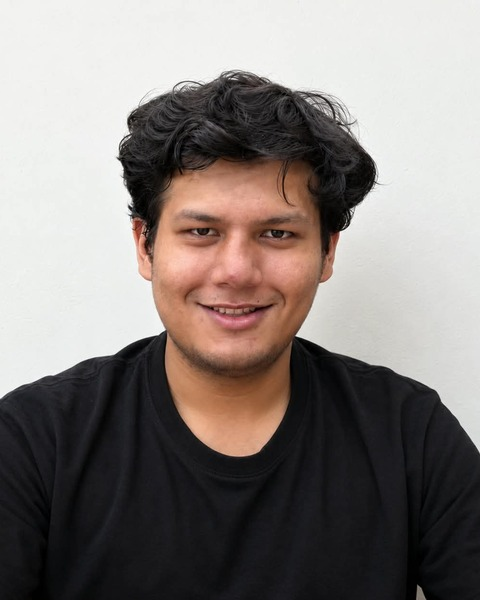
\includegraphics[width=1in,height=1.25in,clip,keepaspectratio]{photos/pancholi.jpg}}]{Parth Pancholi}
is currently pursuing the B.Tech. degree in computer science and engineering with the School of Computing Science and Engineering (SCOPE), VIT Bhopal University, Bhopal, India. He developed the UrbanFix platform presented in this article, including the YOLOv8-based photo screening models, the server-enforced complaint workflow, the public registry, and the research data gateway. His research interests include computer vision, object detection, human-in-the-loop artificial intelligence, civic technology, e-governance, and privacy in data sharing.
\end{IEEEbiography}

\begin{IEEEbiography}[{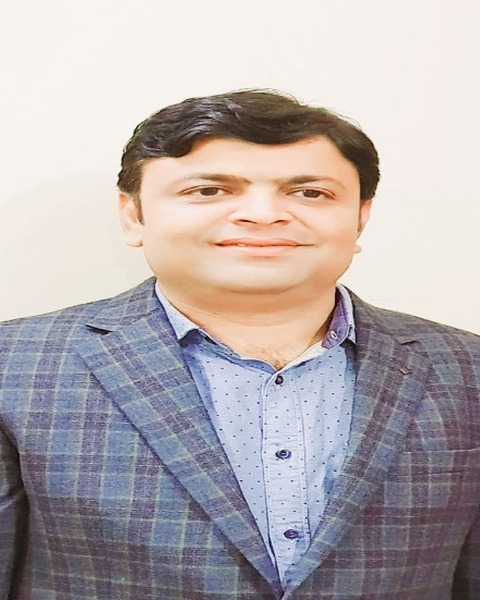
\includegraphics[width=1in,height=1.25in,clip,keepaspectratio]{photos/soni.jpg}}]{Gaurav Soni}
(Senior Member, IEEE) is a Senior Assistant Professor with the School of Computing Science and Engineering (SCOPE), VIT Bhopal University, Bhopal, India. He has 15 years of academic experience. He has published 46 articles in peer-reviewed international and national journals with high impact factors, as well as papers at international conferences held in India and abroad, and he has published six technical patents. His research interests include wireless networks, the Internet of Things (IoT), artificial intelligence, network security, flying ad hoc networks (FANETs), and vehicular ad hoc networks (VANETs).

Dr. Soni is a member of the ACM and holds an associate-level AWS certification.
\end{IEEEbiography}

\begin{IEEEbiography}[{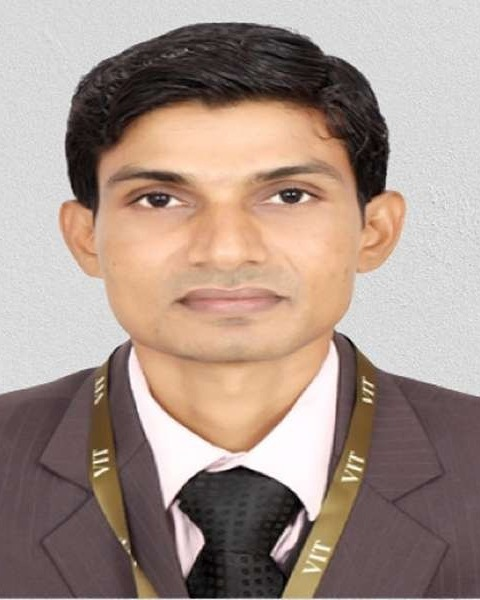
\includegraphics[width=1in,height=1.25in,clip,keepaspectratio]{photos/chandravanshi.jpg}}]{Kamlesh Chandravanshi}
received the M.Tech. and Ph.D. degrees in computer science and engineering. He is currently with the School of Computing Science and Engineering (SCOPE), VIT Bhopal University, Bhopal, India, and has 17 years of academic experience. He has 45 publications in peer-reviewed international and national journals with high impact factors and eight publications at international conferences held in India and abroad. His research interests include mobile ad hoc networks, wireless sensor networks, and the Internet of Things (IoT).

Dr. Chandravanshi serves as a reviewer for several international journals and is a Professional Member of the IACSIT.
\end{IEEEbiography}

\begin{IEEEbiography}[{
\includegraphics[width=1in,height=1.25in,clip,keepaspectratio]{photos/sahare.jpg}}]{Mahendra Sahare}
received the M.Tech. degree in computer science and engineering from RGPV, Bhopal, India, and the Ph.D. degree in computer science and engineering from RNTU, Bhopal. He is currently an Assistant Professor (Senior Grade 1) with the School of Computer Science and Engineering (SCOPE), VIT-AP University, Amaravati, India. He has more than 16 years of academic experience and has served as a Department Head and as the NBA and NAAC Criterion III Coordinator at previous institutions.

He holds three patents, has 12 publications in peer-reviewed international and national journals with high impact factors and six publications at international conferences held in India and abroad, and has published a book on artificial intelligence with Technical Press.

Dr. Sahare is a life member of ARESS and was a member of the ACM Student Chapter and the IIC at his previous institution. He received the Best Faculty Award from the management of NIIST Bhopal.
\end{IEEEbiography}

\begin{IEEEbiography}[{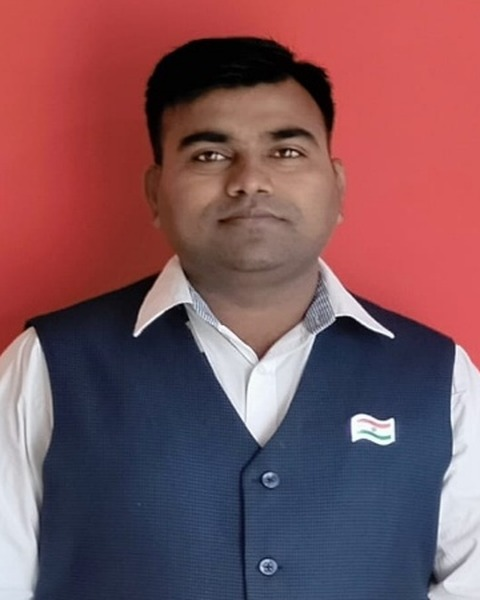
\includegraphics[width=1in,height=1.25in,clip,keepaspectratio]{photos/maurya.jpg}}]{Jay Prakash Maurya}
is currently pursuing the Ph.D. degree with SATI (Autonomous), RGPV, Bhopal, India. He received a postgraduate diploma in system database administration from CDAC, Noida, India. He is currently an Assistant Professor with the School of Computing Science and Engineering (SCOPE), VIT Bhopal University, Bhopal, India, and has 11 years of teaching and research experience. He has published more than 40 research papers in reputed international and national journals and conference proceedings, including Scopus-indexed and UGC-listed venues, and five book chapters in the fields of data mining, image processing, and network security. He also holds three patents and two copyrights. His current research interests include data mining, machine learning, soft computing, and the IoT.

Mr. Maurya is certified in CCNA, CompTIA, and system database administration by CDAC, Noida. He has conducted workshops in collaboration with IIT Bombay for the ``Smart Classroom'' and ``Bodhi Tree'' projects under the Spoken Tutorial initiative.
\end{IEEEbiography}

\EOD

\end{document}
